\documentclass[twoside]{book}

% Packages required by doxygen
\usepackage{fixltx2e}
\usepackage{calc}
\usepackage{doxygen}
\usepackage[export]{adjustbox} % also loads graphicx
\usepackage{graphicx}
\usepackage[utf8]{inputenc}
\usepackage{makeidx}
\usepackage{multicol}
\usepackage{multirow}
\PassOptionsToPackage{warn}{textcomp}
\usepackage{textcomp}
\usepackage[nointegrals]{wasysym}
\usepackage[table]{xcolor}

% Font selection
\usepackage[T1]{fontenc}
\usepackage[scaled=.90]{helvet}
\usepackage{courier}
\usepackage{amssymb}
\usepackage{sectsty}
\renewcommand{\familydefault}{\sfdefault}
\allsectionsfont{%
  \fontseries{bc}\selectfont%
  \color{darkgray}%
}
\renewcommand{\DoxyLabelFont}{%
  \fontseries{bc}\selectfont%
  \color{darkgray}%
}
\newcommand{\+}{\discretionary{\mbox{\scriptsize$\hookleftarrow$}}{}{}}

% Page & text layout
\usepackage{geometry}
\geometry{%
  a4paper,%
  top=2.5cm,%
  bottom=2.5cm,%
  left=2.5cm,%
  right=2.5cm%
}
\tolerance=750
\hfuzz=15pt
\hbadness=750
\setlength{\emergencystretch}{15pt}
\setlength{\parindent}{0cm}
\setlength{\parskip}{3ex plus 2ex minus 2ex}
\makeatletter
\renewcommand{\paragraph}{%
  \@startsection{paragraph}{4}{0ex}{-1.0ex}{1.0ex}{%
    \normalfont\normalsize\bfseries\SS@parafont%
  }%
}
\renewcommand{\subparagraph}{%
  \@startsection{subparagraph}{5}{0ex}{-1.0ex}{1.0ex}{%
    \normalfont\normalsize\bfseries\SS@subparafont%
  }%
}
\makeatother

% Headers & footers
\usepackage{fancyhdr}
\pagestyle{fancyplain}
\fancyhead[LE]{\fancyplain{}{\bfseries\thepage}}
\fancyhead[CE]{\fancyplain{}{}}
\fancyhead[RE]{\fancyplain{}{\bfseries\leftmark}}
\fancyhead[LO]{\fancyplain{}{\bfseries\rightmark}}
\fancyhead[CO]{\fancyplain{}{}}
\fancyhead[RO]{\fancyplain{}{\bfseries\thepage}}
\fancyfoot[LE]{\fancyplain{}{}}
\fancyfoot[CE]{\fancyplain{}{}}
\fancyfoot[RE]{\fancyplain{}{\bfseries\scriptsize Generated by Doxygen }}
\fancyfoot[LO]{\fancyplain{}{\bfseries\scriptsize Generated by Doxygen }}
\fancyfoot[CO]{\fancyplain{}{}}
\fancyfoot[RO]{\fancyplain{}{}}
\renewcommand{\footrulewidth}{0.4pt}
\renewcommand{\chaptermark}[1]{%
  \markboth{#1}{}%
}
\renewcommand{\sectionmark}[1]{%
  \markright{\thesection\ #1}%
}

% Indices & bibliography
\usepackage{natbib}
\usepackage[titles]{tocloft}
\setcounter{tocdepth}{3}
\setcounter{secnumdepth}{5}
\makeindex

% Hyperlinks (required, but should be loaded last)
\usepackage{ifpdf}
\ifpdf
  \usepackage[pdftex,pagebackref=true]{hyperref}
\else
  \usepackage[ps2pdf,pagebackref=true]{hyperref}
\fi
\hypersetup{%
  colorlinks=true,%
  linkcolor=blue,%
  citecolor=blue,%
  unicode%
}

% Custom commands
\newcommand{\clearemptydoublepage}{%
  \newpage{\pagestyle{empty}\cleardoublepage}%
}

\usepackage{caption}
\captionsetup{labelsep=space,justification=centering,font={bf},singlelinecheck=off,skip=4pt,position=top}

%===== C O N T E N T S =====

\begin{document}

% Titlepage & ToC
\hypersetup{pageanchor=false,
             bookmarksnumbered=true,
             pdfencoding=unicode
            }
\pagenumbering{alph}
\begin{titlepage}
\vspace*{7cm}
\begin{center}%
{\Large My Project }\\
\vspace*{1cm}
{\large Generated by Doxygen 1.8.13}\\
\end{center}
\end{titlepage}
\clearemptydoublepage
\pagenumbering{roman}
\tableofcontents
\clearemptydoublepage
\pagenumbering{arabic}
\hypersetup{pageanchor=true}

%--- Begin generated contents ---
\chapter{Tetris}
\label{md_README}
\Hypertarget{md_README}
\hyperlink{classJeu}{Jeu} Tetris à développer Librairies à télécharger \+:
\begin{DoxyItemize}
\item ncurses
\end{DoxyItemize}

Pour compiler le programme \+: g++ main.\+cpp -\/lncurses 
\chapter{Bug List}
\label{bug}
\Hypertarget{bug}

\begin{DoxyRefList}
\item[\label{bug__bug000001}%
\Hypertarget{bug__bug000001}%
Class \hyperlink{class_jeu}{Jeu} ]Rien à signaler 
\end{DoxyRefList}
\chapter{Hierarchical Index}
\section{Class Hierarchy}
This inheritance list is sorted roughly, but not completely, alphabetically\+:\begin{DoxyCompactList}
\item \contentsline{section}{Bloc}{\pageref{classBloc}}{}
\item \contentsline{section}{Board}{\pageref{classBoard}}{}
\item \contentsline{section}{I\+HM}{\pageref{classIHM}}{}
\item \contentsline{section}{Jeu}{\pageref{classJeu}}{}
\begin{DoxyCompactList}
\item \contentsline{section}{Jeu\+Classique}{\pageref{classJeuClassique}}{}
\item \contentsline{section}{Jeu\+Montagnard}{\pageref{classJeuMontagnard}}{}
\end{DoxyCompactList}
\item \contentsline{section}{Personnage}{\pageref{classPersonnage}}{}
\item \contentsline{section}{Piece}{\pageref{classPiece}}{}
\begin{DoxyCompactList}
\item \contentsline{section}{Piece\+\_\+I}{\pageref{classPiece__I}}{}
\item \contentsline{section}{Piece\+\_\+J}{\pageref{classPiece__J}}{}
\item \contentsline{section}{Piece\+\_\+L}{\pageref{classPiece__L}}{}
\item \contentsline{section}{Piece\+\_\+O}{\pageref{classPiece__O}}{}
\item \contentsline{section}{Piece\+\_\+S}{\pageref{classPiece__S}}{}
\item \contentsline{section}{Piece\+\_\+T}{\pageref{classPiece__T}}{}
\item \contentsline{section}{Piece\+\_\+Z}{\pageref{classPiece__Z}}{}
\end{DoxyCompactList}
\item \contentsline{section}{Score}{\pageref{classScore}}{}
\end{DoxyCompactList}

\chapter{Class Index}
\section{Class List}
Here are the classes, structs, unions and interfaces with brief descriptions\+:\begin{DoxyCompactList}
\item\contentsline{section}{\hyperlink{classBloc}{Bloc} \\*Représentation d\textquotesingle{}un élément dans l\textquotesingle{}espace }{\pageref{classBloc}}{}
\item\contentsline{section}{\hyperlink{classBoard}{Board} \\*Représentation d\textquotesingle{}une grille de jeu }{\pageref{classBoard}}{}
\item\contentsline{section}{\hyperlink{classIHM}{I\+HM} \\*Gère les interactions entre les actions du joueur et le jeu à proprement parler }{\pageref{classIHM}}{}
\item\contentsline{section}{\hyperlink{classJeu}{Jeu} \\*Gestion du déroulement d\textquotesingle{}une partie }{\pageref{classJeu}}{}
\item\contentsline{section}{\hyperlink{classJeuClassique}{Jeu\+Classique} \\*Gestion du déroulement d\textquotesingle{}un \hyperlink{classJeu}{Jeu} Classique }{\pageref{classJeuClassique}}{}
\item\contentsline{section}{\hyperlink{classJeuMontagnard}{Jeu\+Montagnard} \\*Gestion du déroulement d\textquotesingle{}un \hyperlink{classJeu}{Jeu} Montagnard }{\pageref{classJeuMontagnard}}{}
\item\contentsline{section}{\hyperlink{classMenu}{Menu} }{\pageref{classMenu}}{}
\item\contentsline{section}{\hyperlink{classPersonnage}{Personnage} \\*Représentation du \hyperlink{classPersonnage}{Personnage} pour la version montagnarde du Tetris }{\pageref{classPersonnage}}{}
\item\contentsline{section}{\hyperlink{classPiece}{Piece} \\*Représentation d\textquotesingle{}une \hyperlink{classPiece}{Piece} de jeu }{\pageref{classPiece}}{}
\item\contentsline{section}{\hyperlink{classPiece__I}{Piece\+\_\+I} \\*Représentation d\textquotesingle{}un Tétrimino en forme de I. Hérite de \hyperlink{classPiece}{Piece} }{\pageref{classPiece__I}}{}
\item\contentsline{section}{\hyperlink{classPiece__J}{Piece\+\_\+J} \\*Représentation d\textquotesingle{}un Tétrimino en forme de J. Hérite de \hyperlink{classPiece}{Piece} }{\pageref{classPiece__J}}{}
\item\contentsline{section}{\hyperlink{classPiece__L}{Piece\+\_\+L} \\*Représentation d\textquotesingle{}un Tétrimino en forme de L. Hérite de \hyperlink{classPiece}{Piece} }{\pageref{classPiece__L}}{}
\item\contentsline{section}{\hyperlink{classPiece__O}{Piece\+\_\+O} \\*Représentation d\textquotesingle{}un Tétrimino en forme de carré. Hérite de \hyperlink{classPiece}{Piece} }{\pageref{classPiece__O}}{}
\item\contentsline{section}{\hyperlink{classPiece__S}{Piece\+\_\+S} \\*Représentation d\textquotesingle{}un Tétrimino en forme de S. Hérite de \hyperlink{classPiece}{Piece} }{\pageref{classPiece__S}}{}
\item\contentsline{section}{\hyperlink{classPiece__T}{Piece\+\_\+T} \\*Représentation d\textquotesingle{}un Tétrimino en forme de T. Hérite de \hyperlink{classPiece}{Piece} }{\pageref{classPiece__T}}{}
\item\contentsline{section}{\hyperlink{classPiece__Z}{Piece\+\_\+Z} \\*Représentation d\textquotesingle{}un Tétrimino en forme de J. Hérite de \hyperlink{classPiece}{Piece} }{\pageref{classPiece__Z}}{}
\item\contentsline{section}{\hyperlink{classScore}{Score} \\*Gestion des meilleurs \hyperlink{classScore}{Score} des joueurs }{\pageref{classScore}}{}
\end{DoxyCompactList}

\chapter{Class Documentation}
\hypertarget{classBloc}{}\section{Bloc Class Reference}
\label{classBloc}\index{Bloc@{Bloc}}


Représentation d\textquotesingle{}un élément dans l\textquotesingle{}espace.  




{\ttfamily \#include $<$Bloc.\+hpp$>$}

\subsection*{Public Member Functions}
\begin{DoxyCompactItemize}
\item 
\mbox{\Hypertarget{classBloc_a67d18e588715a983cf7980ae23d9e939}\label{classBloc_a67d18e588715a983cf7980ae23d9e939}} 
{\bfseries Bloc} (int x, int y)
\item 
int \hyperlink{classBloc_a1600764b66f921e77cb5ca8d2946a3e2}{get\+Posx} () const
\item 
int \hyperlink{classBloc_a362522a2a75cefdbba44a544cd7f1a75}{get\+Posy} () const
\item 
void \hyperlink{classBloc_a2d50fb680c5b8d3d3de2566a125d25a2}{set\+Posx} (int x)
\begin{DoxyCompactList}\small\item\em modifie la position en abscisse d\textquotesingle{}un bloc \end{DoxyCompactList}\item 
void \hyperlink{classBloc_a361647f817b1f6202ee29c77e8f03f79}{set\+Posy} (int y)
\begin{DoxyCompactList}\small\item\em modifie la position en ordonnée d\textquotesingle{}un bloc \end{DoxyCompactList}\end{DoxyCompactItemize}


\subsection{Detailed Description}
Représentation d\textquotesingle{}un élément dans l\textquotesingle{}espace. 

\begin{DoxyAuthor}{Author}
Victor Le Maistre 
\end{DoxyAuthor}
\begin{DoxyVersion}{Version}
1.\+0 
\end{DoxyVersion}
\begin{DoxyDate}{Date}
avril 2018 
\end{DoxyDate}
\begin{DoxyRefDesc}{Bug}
\item[\hyperlink{bug__bug000001}{Bug}]Rien à signaler \end{DoxyRefDesc}
\begin{DoxyWarning}{Warning}
Rien à signaler
\end{DoxyWarning}
Ce module permet de représenter un élément dans l\textquotesingle{}espace, par sa position en x et sa position en y. On pourra modifier ces positions. 

\subsection{Member Function Documentation}
\mbox{\Hypertarget{classBloc_a1600764b66f921e77cb5ca8d2946a3e2}\label{classBloc_a1600764b66f921e77cb5ca8d2946a3e2}} 
\index{Bloc@{Bloc}!get\+Posx@{get\+Posx}}
\index{get\+Posx@{get\+Posx}!Bloc@{Bloc}}
\subsubsection{\texorpdfstring{get\+Posx()}{getPosx()}}
{\footnotesize\ttfamily int Bloc\+::get\+Posx (\begin{DoxyParamCaption}{ }\end{DoxyParamCaption}) const}

\begin{DoxyReturn}{Returns}
renvoie la position en abscisse d\textquotesingle{}un bloc 
\end{DoxyReturn}
\mbox{\Hypertarget{classBloc_a362522a2a75cefdbba44a544cd7f1a75}\label{classBloc_a362522a2a75cefdbba44a544cd7f1a75}} 
\index{Bloc@{Bloc}!get\+Posy@{get\+Posy}}
\index{get\+Posy@{get\+Posy}!Bloc@{Bloc}}
\subsubsection{\texorpdfstring{get\+Posy()}{getPosy()}}
{\footnotesize\ttfamily int Bloc\+::get\+Posy (\begin{DoxyParamCaption}{ }\end{DoxyParamCaption}) const}

\begin{DoxyReturn}{Returns}
renvoie la position en ordonnée d\textquotesingle{}un bloc 
\end{DoxyReturn}
\mbox{\Hypertarget{classBloc_a2d50fb680c5b8d3d3de2566a125d25a2}\label{classBloc_a2d50fb680c5b8d3d3de2566a125d25a2}} 
\index{Bloc@{Bloc}!set\+Posx@{set\+Posx}}
\index{set\+Posx@{set\+Posx}!Bloc@{Bloc}}
\subsubsection{\texorpdfstring{set\+Posx()}{setPosx()}}
{\footnotesize\ttfamily void Bloc\+::set\+Posx (\begin{DoxyParamCaption}\item[{int}]{x }\end{DoxyParamCaption})}



modifie la position en abscisse d\textquotesingle{}un bloc 


\begin{DoxyParams}{Parameters}
{\em x} & correspond à la position que l\textquotesingle{}on veut en abscisse en sortie de cette fonction \\
\hline
\end{DoxyParams}
\mbox{\Hypertarget{classBloc_a361647f817b1f6202ee29c77e8f03f79}\label{classBloc_a361647f817b1f6202ee29c77e8f03f79}} 
\index{Bloc@{Bloc}!set\+Posy@{set\+Posy}}
\index{set\+Posy@{set\+Posy}!Bloc@{Bloc}}
\subsubsection{\texorpdfstring{set\+Posy()}{setPosy()}}
{\footnotesize\ttfamily void Bloc\+::set\+Posy (\begin{DoxyParamCaption}\item[{int}]{y }\end{DoxyParamCaption})}



modifie la position en ordonnée d\textquotesingle{}un bloc 


\begin{DoxyParams}{Parameters}
{\em y} & correspond à la position que l\textquotesingle{}on veut en ordonnée en sortie de cette fonction \\
\hline
\end{DoxyParams}


The documentation for this class was generated from the following files\+:\begin{DoxyCompactItemize}
\item 
Bloc.\+hpp\item 
Bloc.\+cpp\end{DoxyCompactItemize}

\hypertarget{classBoard}{}\section{Board Class Reference}
\label{classBoard}\index{Board@{Board}}


Représentation d\textquotesingle{}une grille de jeu.  




{\ttfamily \#include $<$Board.\+hpp$>$}

\subsection*{Public Member Functions}
\begin{DoxyCompactItemize}
\item 
\mbox{\Hypertarget{classBoard_ac7cfff6987702708f85280af70e6c7b4}\label{classBoard_ac7cfff6987702708f85280af70e6c7b4}} 
int \hyperlink{classBoard_ac7cfff6987702708f85280af70e6c7b4}{get\+Largeur} () const
\begin{DoxyCompactList}\small\item\em renvoie la largeur de la grille, c\textquotesingle{}est-\/à-\/dire le nombre de colonnes \end{DoxyCompactList}\item 
\mbox{\Hypertarget{classBoard_af69f2b14974e2c6b7fcffa3fef58340f}\label{classBoard_af69f2b14974e2c6b7fcffa3fef58340f}} 
int \hyperlink{classBoard_af69f2b14974e2c6b7fcffa3fef58340f}{get\+Hauteur} () const
\begin{DoxyCompactList}\small\item\em renvoie la hauteur de la grille, c\textquotesingle{}est-\/à-\/dire le nombre de lignes \end{DoxyCompactList}\item 
\mbox{\Hypertarget{classBoard_aea48e2901225f0fae6af38096fb16ef8}\label{classBoard_aea48e2901225f0fae6af38096fb16ef8}} 
int \hyperlink{classBoard_aea48e2901225f0fae6af38096fb16ef8}{get\+Grille} (int x, int y) const
\begin{DoxyCompactList}\small\item\em renvoie l\textquotesingle{}élément de la grille se situant à x en abscisse, y en ordonnée. \end{DoxyCompactList}\item 
\mbox{\Hypertarget{classBoard_a7c06f0c081a6a037fa65204a7a9badd2}\label{classBoard_a7c06f0c081a6a037fa65204a7a9badd2}} 
void \hyperlink{classBoard_a7c06f0c081a6a037fa65204a7a9badd2}{set\+Grille} (int x, int y)
\begin{DoxyCompactList}\small\item\em modifie la valeur de la grille dans la case en \mbox{[}x,y\mbox{]} \end{DoxyCompactList}\item 
\mbox{\Hypertarget{classBoard_a2cf5d799795f86a50d5d6eb4bd353b93}\label{classBoard_a2cf5d799795f86a50d5d6eb4bd353b93}} 
void \hyperlink{classBoard_a2cf5d799795f86a50d5d6eb4bd353b93}{init} ()
\begin{DoxyCompactList}\small\item\em initialise une grille en début de \hyperlink{classJeu}{Jeu} en la remplissant de 0 \end{DoxyCompactList}\end{DoxyCompactItemize}
\subsection*{Friends}
\begin{DoxyCompactItemize}
\item 
\mbox{\Hypertarget{classBoard_aa4c1980eaf4ad187b9af05d10567dae3}\label{classBoard_aa4c1980eaf4ad187b9af05d10567dae3}} 
ostream \& \hyperlink{classBoard_aa4c1980eaf4ad187b9af05d10567dae3}{operator$<$$<$} (ostream \&out, \hyperlink{classBoard}{Board} \&)
\begin{DoxyCompactList}\small\item\em Cette classe ami permet d\textquotesingle{}afficher la grille sur un terminal, affiche un x lorsque la grille comprend un 1, et affiche 0 sinon. \end{DoxyCompactList}\end{DoxyCompactItemize}


\subsection{Detailed Description}
Représentation d\textquotesingle{}une grille de jeu. 

\begin{DoxyAuthor}{Author}
Victor Le Maistre 
\end{DoxyAuthor}
\begin{DoxyVersion}{Version}
1.\+0 
\end{DoxyVersion}
\begin{DoxyDate}{Date}
avril 2018 
\end{DoxyDate}
\begin{DoxyRefDesc}{Bug}
\item[\hyperlink{bug__bug000002}{Bug}]Rien à signaler \end{DoxyRefDesc}
\begin{DoxyWarning}{Warning}
Rien à signaler
\end{DoxyWarning}
Ce module permet de représenter une grille de jeu dont on peut choisir la dimension en largeur (horizontalement) et en hauteur (verticalement). On pourra modifier la largeur et la hauteur de cette grille. Un élément de la grille vaut 1 s\textquotesingle{}il contient quelque chose, 0 sinon. Pour finir, on pourra avoir accès et modifier les éléments de la grille. 

The documentation for this class was generated from the following files\+:\begin{DoxyCompactItemize}
\item 
Board.\+hpp\item 
Board.\+cpp\end{DoxyCompactItemize}

\hypertarget{classIHM}{}\section{I\+HM Class Reference}
\label{classIHM}\index{I\+HM@{I\+HM}}


Gère les interactions entre les actions du joueur et le jeu à proprement parler.  




{\ttfamily \#include $<$I\+H\+M.\+hpp$>$}

\subsection*{Static Public Member Functions}
\begin{DoxyCompactItemize}
\item 
static int \hyperlink{classIHM_a87654cde450f04cacddaf7a781f5300c}{getinput} ()
\begin{DoxyCompactList}\small\item\em Récupère les données saisies par l\textquotesingle{}utilisateur sur le clavier. \end{DoxyCompactList}\item 
static void \hyperlink{classIHM_a48abb3aee5c33a71f6fc2c3528f99afb}{afficher} (\hyperlink{classBoard}{Board} b, \hyperlink{classPiece}{Piece} $\ast$Piece\+En\+Cours, \hyperlink{classPiece}{Piece} $\ast$Piece\+Stockee, \hyperlink{classPiece}{Piece} $\ast$Piece\+Suivante, int \hyperlink{classScore}{Score}, bool pause)
\begin{DoxyCompactList}\small\item\em Affiche l\textquotesingle{}interface graphique du Tetris Classique en fonction de l\textquotesingle{}état courant du jeu. \end{DoxyCompactList}\item 
static void \hyperlink{classIHM_afe38f71bf414ddd7e934174657c175e3}{afficher} (\hyperlink{classBoard}{Board} b, \hyperlink{classPiece}{Piece} $\ast$Piece\+En\+Cours, \hyperlink{classPiece}{Piece} $\ast$Piece\+Stockee, \hyperlink{classPiece}{Piece} $\ast$Piece\+Suivante, int \hyperlink{classScore}{Score}, bool pause, \hyperlink{classPersonnage}{Personnage} p)
\begin{DoxyCompactList}\small\item\em Affiche l\textquotesingle{}interface graphique du Tetris Montagnard en fonction de l\textquotesingle{}état courant du jeu. \end{DoxyCompactList}\item 
\mbox{\Hypertarget{classIHM_a05f1daa32a6db641f74c5d6083c33743}\label{classIHM_a05f1daa32a6db641f74c5d6083c33743}} 
static void \hyperlink{classIHM_a05f1daa32a6db641f74c5d6083c33743}{menu} ()
\begin{DoxyCompactList}\small\item\em Affiche le menu d\textquotesingle{}accueil de notre application. \end{DoxyCompactList}\item 
\mbox{\Hypertarget{classIHM_a79d4bc8301e8a664c9bfea8d0b2ca916}\label{classIHM_a79d4bc8301e8a664c9bfea8d0b2ca916}} 
static void \hyperlink{classIHM_a79d4bc8301e8a664c9bfea8d0b2ca916}{score} ()
\begin{DoxyCompactList}\small\item\em Affiche tous les meilleurs scores (\hyperlink{classJeu}{Jeu} Classique et \hyperlink{classJeu}{Jeu} Montagnard) \end{DoxyCompactList}\item 
\mbox{\Hypertarget{classIHM_a41f84c5e14ce96d0dc25a42fe214bf3f}\label{classIHM_a41f84c5e14ce96d0dc25a42fe214bf3f}} 
static void \hyperlink{classIHM_a41f84c5e14ce96d0dc25a42fe214bf3f}{reglesdu\+Jeu} ()
\begin{DoxyCompactList}\small\item\em Affiche les règles du jeu. \end{DoxyCompactList}\item 
\mbox{\Hypertarget{classIHM_ac2e668b4fa5ff1491bc15ae0a2d59d1d}\label{classIHM_ac2e668b4fa5ff1491bc15ae0a2d59d1d}} 
static void \hyperlink{classIHM_ac2e668b4fa5ff1491bc15ae0a2d59d1d}{Score\+Classique} ()
\begin{DoxyCompactList}\small\item\em Affiche les meilleurs scores des parties classiques. \end{DoxyCompactList}\item 
\mbox{\Hypertarget{classIHM_a8f4dce1d816518f673fcafca08fd0ce5}\label{classIHM_a8f4dce1d816518f673fcafca08fd0ce5}} 
static void \hyperlink{classIHM_a8f4dce1d816518f673fcafca08fd0ce5}{Score\+Montagnard} ()
\begin{DoxyCompactList}\small\item\em Affiche les meilleurs scores des parties montagnardes. \end{DoxyCompactList}\item 
static int \hyperlink{classIHM_a4218e5b720799dd8bada264c7bc0d690}{Meilleur\+Score\+Classique} (int)
\begin{DoxyCompactList}\small\item\em Récupère le sième meilleure score des parties classiques. \end{DoxyCompactList}\item 
static int \hyperlink{classIHM_a068cc2350e9f4fc005ad4378f02d62fa}{Meilleur\+Score\+Montagnard} (int s)
\begin{DoxyCompactList}\small\item\em Récupère le sième meilleure score des parties montagnardes. \end{DoxyCompactList}\end{DoxyCompactItemize}


\subsection{Detailed Description}
Gère les interactions entre les actions du joueur et le jeu à proprement parler. 

\begin{DoxyAuthor}{Author}
Léa Lefrançois 

Laura Couret 

Victor Le Maistre 
\end{DoxyAuthor}
\begin{DoxyVersion}{Version}
1.\+0 
\end{DoxyVersion}
\begin{DoxyDate}{Date}
avril 2018 
\end{DoxyDate}
\begin{DoxyRefDesc}{Bug}
\item[\hyperlink{bug__bug000003}{Bug}]Rien à signaler \end{DoxyRefDesc}
\begin{DoxyWarning}{Warning}
Rien à signaler
\end{DoxyWarning}
Ce module va permettre de \+:
\begin{DoxyItemize}
\item récupérer les saisies clavier de l\textquotesingle{}utilisateur
\item afficher le menu
\item afficher une interface graphique du jeu
\item afficher les scores et les règles du jeu
\item consulter et ajouter des meilleurs scores autant pour le jeu Classique que le Montagnard 
\end{DoxyItemize}

\subsection{Member Function Documentation}
\mbox{\Hypertarget{classIHM_a48abb3aee5c33a71f6fc2c3528f99afb}\label{classIHM_a48abb3aee5c33a71f6fc2c3528f99afb}} 
\index{I\+HM@{I\+HM}!afficher@{afficher}}
\index{afficher@{afficher}!I\+HM@{I\+HM}}
\subsubsection{\texorpdfstring{afficher()}{afficher()}\hspace{0.1cm}{\footnotesize\ttfamily [1/2]}}
{\footnotesize\ttfamily static void I\+H\+M\+::afficher (\begin{DoxyParamCaption}\item[{\hyperlink{classBoard}{Board}}]{b,  }\item[{\hyperlink{classPiece}{Piece} $\ast$}]{Piece\+En\+Cours,  }\item[{\hyperlink{classPiece}{Piece} $\ast$}]{Piece\+Stockee,  }\item[{\hyperlink{classPiece}{Piece} $\ast$}]{Piece\+Suivante,  }\item[{int}]{Score,  }\item[{bool}]{Pause }\end{DoxyParamCaption})\hspace{0.3cm}{\ttfamily [static]}}



Affiche l\textquotesingle{}interface graphique du Tetris Classique en fonction de l\textquotesingle{}état courant du jeu. 


\begin{DoxyParams}{Parameters}
{\em b} & est la grille de jeu \\
\hline
{\em $\ast$\+Piece\+En\+Cours} & est le pointeur sur la Pièce actuellement en train de descendre le long de la grille de jeu \\
\hline
{\em $\ast$\+Piece\+Stockee} & est le pointeur sur la Pièce actuellement stockée par le joueur \\
\hline
{\em $\ast$\+Piece\+Suivante} & est le pointeur sur la prochaine Pièce à descendre le long de la grille de jeu \\
\hline
{\em \hyperlink{classScore}{Score}} & est le score actuel du joueur en points \\
\hline
{\em bool} & est le booleen qui permet de savoir si on affiche le jeu, ou si on affiche un message de pause \\
\hline
\end{DoxyParams}
\mbox{\Hypertarget{classIHM_afe38f71bf414ddd7e934174657c175e3}\label{classIHM_afe38f71bf414ddd7e934174657c175e3}} 
\index{I\+HM@{I\+HM}!afficher@{afficher}}
\index{afficher@{afficher}!I\+HM@{I\+HM}}
\subsubsection{\texorpdfstring{afficher()}{afficher()}\hspace{0.1cm}{\footnotesize\ttfamily [2/2]}}
{\footnotesize\ttfamily static void I\+H\+M\+::afficher (\begin{DoxyParamCaption}\item[{\hyperlink{classBoard}{Board}}]{b,  }\item[{\hyperlink{classPiece}{Piece} $\ast$}]{Piece\+En\+Cours,  }\item[{\hyperlink{classPiece}{Piece} $\ast$}]{Piece\+Stockee,  }\item[{\hyperlink{classPiece}{Piece} $\ast$}]{Piece\+Suivante,  }\item[{int}]{Score,  }\item[{bool}]{pause,  }\item[{\hyperlink{classPersonnage}{Personnage}}]{p }\end{DoxyParamCaption})\hspace{0.3cm}{\ttfamily [static]}}



Affiche l\textquotesingle{}interface graphique du Tetris Montagnard en fonction de l\textquotesingle{}état courant du jeu. 


\begin{DoxyParams}{Parameters}
{\em b} & est la grille de jeu \\
\hline
{\em $\ast$\+Piece\+En\+Cours} & est le pointeur sur la Pièce actuellement en train de descendre le long de la grille de jeu \\
\hline
{\em $\ast$\+Piece\+Stockee} & est le pointeur sur la Pièce actuellement stockée par le joueur \\
\hline
{\em $\ast$\+Piece\+Suivante} & est le pointeur sur la prochaine Pièce à descendre le long de la grille de jeu \\
\hline
{\em \hyperlink{classScore}{Score}} & est le score actuel du joueur en millisecondes \\
\hline
{\em bool} & est le booleen qui permet de savoir si on affiche le jeu, ou si on affiche un message de pause \\
\hline
{\em p} & est le \hyperlink{classPersonnage}{Personnage} du Tetris Montagnard \\
\hline
\end{DoxyParams}
\mbox{\Hypertarget{classIHM_a87654cde450f04cacddaf7a781f5300c}\label{classIHM_a87654cde450f04cacddaf7a781f5300c}} 
\index{I\+HM@{I\+HM}!getinput@{getinput}}
\index{getinput@{getinput}!I\+HM@{I\+HM}}
\subsubsection{\texorpdfstring{getinput()}{getinput()}}
{\footnotesize\ttfamily static int I\+H\+M\+::getinput (\begin{DoxyParamCaption}{ }\end{DoxyParamCaption})\hspace{0.3cm}{\ttfamily [static]}}



Récupère les données saisies par l\textquotesingle{}utilisateur sur le clavier. 

\begin{DoxyReturn}{Returns}
l\textquotesingle{}entier correspondant au caractère tapé 
\end{DoxyReturn}
\mbox{\Hypertarget{classIHM_a4218e5b720799dd8bada264c7bc0d690}\label{classIHM_a4218e5b720799dd8bada264c7bc0d690}} 
\index{I\+HM@{I\+HM}!Meilleur\+Score\+Classique@{Meilleur\+Score\+Classique}}
\index{Meilleur\+Score\+Classique@{Meilleur\+Score\+Classique}!I\+HM@{I\+HM}}
\subsubsection{\texorpdfstring{Meilleur\+Score\+Classique()}{MeilleurScoreClassique()}}
{\footnotesize\ttfamily static int I\+H\+M\+::\+Meilleur\+Score\+Classique (\begin{DoxyParamCaption}\item[{int}]{s }\end{DoxyParamCaption})\hspace{0.3cm}{\ttfamily [static]}}



Récupère le sième meilleure score des parties classiques. 


\begin{DoxyParams}{Parameters}
{\em s} & le numéro du score que l\textquotesingle{}on veut afficher, doit être compris entre 1 et 5 \\
\hline
\end{DoxyParams}
\begin{DoxyReturn}{Returns}
Retourne le sième meilleure score des parties classiques 
\end{DoxyReturn}
\mbox{\Hypertarget{classIHM_a068cc2350e9f4fc005ad4378f02d62fa}\label{classIHM_a068cc2350e9f4fc005ad4378f02d62fa}} 
\index{I\+HM@{I\+HM}!Meilleur\+Score\+Montagnard@{Meilleur\+Score\+Montagnard}}
\index{Meilleur\+Score\+Montagnard@{Meilleur\+Score\+Montagnard}!I\+HM@{I\+HM}}
\subsubsection{\texorpdfstring{Meilleur\+Score\+Montagnard()}{MeilleurScoreMontagnard()}}
{\footnotesize\ttfamily static int I\+H\+M\+::\+Meilleur\+Score\+Montagnard (\begin{DoxyParamCaption}\item[{int}]{s }\end{DoxyParamCaption})\hspace{0.3cm}{\ttfamily [static]}}



Récupère le sième meilleure score des parties montagnardes. 


\begin{DoxyParams}{Parameters}
{\em s} & le numéro du score que l\textquotesingle{}on veut afficher, doit être compris entre 1 et 5 \\
\hline
\end{DoxyParams}
\begin{DoxyReturn}{Returns}
Retourne le sième meilleure score des parties montagnardes 
\end{DoxyReturn}


The documentation for this class was generated from the following files\+:\begin{DoxyCompactItemize}
\item 
I\+H\+M.\+hpp\item 
I\+H\+M.\+cpp\end{DoxyCompactItemize}

\hypertarget{classJeu}{}\section{Jeu Class Reference}
\label{classJeu}\index{Jeu@{Jeu}}


Gestion du déroulement d\textquotesingle{}une partie.  




{\ttfamily \#include $<$Jeu.\+hpp$>$}



Inheritance diagram for Jeu\+:
\nopagebreak
\begin{figure}[H]
\begin{center}
\leavevmode
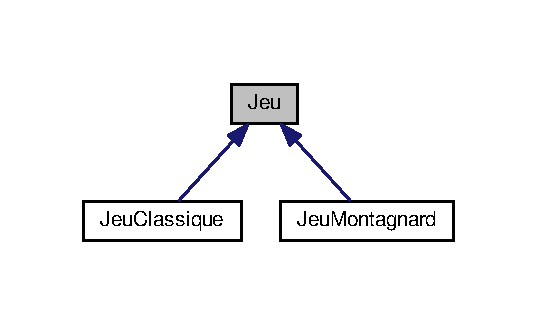
\includegraphics[width=258pt]{classJeu__inherit__graph}
\end{center}
\end{figure}
\subsection*{Public Member Functions}
\begin{DoxyCompactItemize}
\item 
\mbox{\Hypertarget{classJeu_a16a1b627ca2c860ab3e6ed90111619d0}\label{classJeu_a16a1b627ca2c860ab3e6ed90111619d0}} 
void \hyperlink{classJeu_a16a1b627ca2c860ab3e6ed90111619d0}{MaJ} ()
\begin{DoxyCompactList}\small\item\em Met à jour la grille à chaque fois qu\textquotesingle{}une pièce est posée. \end{DoxyCompactList}\item 
\mbox{\Hypertarget{classJeu_a511f7634136222441ecb3b64a408b505}\label{classJeu_a511f7634136222441ecb3b64a408b505}} 
bool {\bfseries getjeu} () const
\item 
\mbox{\Hypertarget{classJeu_a590b59debf5cf7906dba4bce371b2c16}\label{classJeu_a590b59debf5cf7906dba4bce371b2c16}} 
bool {\bfseries getstatut} ()
\item 
\mbox{\Hypertarget{classJeu_a0ad85d37e6ffc90d919440a13404fae3}\label{classJeu_a0ad85d37e6ffc90d919440a13404fae3}} 
void {\bfseries interaction} (int c)
\item 
\mbox{\Hypertarget{classJeu_af8832b6cdb31f97f5dec8ed4e38a5200}\label{classJeu_af8832b6cdb31f97f5dec8ed4e38a5200}} 
void \hyperlink{classJeu_af8832b6cdb31f97f5dec8ed4e38a5200}{init} ()
\begin{DoxyCompactList}\small\item\em Initialise le jeu en début de partie. \end{DoxyCompactList}\item 
\mbox{\Hypertarget{classJeu_ad339f827f08dabcb27a90844822b268e}\label{classJeu_ad339f827f08dabcb27a90844822b268e}} 
void \hyperlink{classJeu_ad339f827f08dabcb27a90844822b268e}{play} ()
\begin{DoxyCompactList}\small\item\em Contient la boucle principale qui fait tourner le \hyperlink{classJeu}{Jeu}. \end{DoxyCompactList}\item 
\mbox{\Hypertarget{classJeu_a16a1b627ca2c860ab3e6ed90111619d0}\label{classJeu_a16a1b627ca2c860ab3e6ed90111619d0}} 
void {\bfseries MaJ} ()
\item 
\mbox{\Hypertarget{classJeu_af8832b6cdb31f97f5dec8ed4e38a5200}\label{classJeu_af8832b6cdb31f97f5dec8ed4e38a5200}} 
void {\bfseries init} ()
\item 
\mbox{\Hypertarget{classJeu_ad339f827f08dabcb27a90844822b268e}\label{classJeu_ad339f827f08dabcb27a90844822b268e}} 
void {\bfseries play} ()
\item 
\mbox{\Hypertarget{classJeu_a16a1b627ca2c860ab3e6ed90111619d0}\label{classJeu_a16a1b627ca2c860ab3e6ed90111619d0}} 
void {\bfseries MaJ} ()
\item 
\mbox{\Hypertarget{classJeu_afe5b195769def6b3fdffea8ecf2b090a}\label{classJeu_afe5b195769def6b3fdffea8ecf2b090a}} 
void {\bfseries move} (int c)
\item 
\mbox{\Hypertarget{classJeu_a54a25003d167335db122efb513f6508f}\label{classJeu_a54a25003d167335db122efb513f6508f}} 
void {\bfseries afficher} ()
\item 
\mbox{\Hypertarget{classJeu_af8832b6cdb31f97f5dec8ed4e38a5200}\label{classJeu_af8832b6cdb31f97f5dec8ed4e38a5200}} 
void {\bfseries init} ()
\item 
\mbox{\Hypertarget{classJeu_ad339f827f08dabcb27a90844822b268e}\label{classJeu_ad339f827f08dabcb27a90844822b268e}} 
void {\bfseries play} ()
\item 
\mbox{\Hypertarget{classJeu_a16a1b627ca2c860ab3e6ed90111619d0}\label{classJeu_a16a1b627ca2c860ab3e6ed90111619d0}} 
void {\bfseries MaJ} ()
\item 
\mbox{\Hypertarget{classJeu_a0ad85d37e6ffc90d919440a13404fae3}\label{classJeu_a0ad85d37e6ffc90d919440a13404fae3}} 
void {\bfseries interaction} (int c)
\item 
\mbox{\Hypertarget{classJeu_aa77bc2630c3c090f1eda2b16126a6e43}\label{classJeu_aa77bc2630c3c090f1eda2b16126a6e43}} 
void {\bfseries pause} ()
\item 
\mbox{\Hypertarget{classJeu_af8832b6cdb31f97f5dec8ed4e38a5200}\label{classJeu_af8832b6cdb31f97f5dec8ed4e38a5200}} 
void {\bfseries init} ()
\item 
\mbox{\Hypertarget{classJeu_ad339f827f08dabcb27a90844822b268e}\label{classJeu_ad339f827f08dabcb27a90844822b268e}} 
void {\bfseries play} ()
\item 
\mbox{\Hypertarget{classJeu_a16a1b627ca2c860ab3e6ed90111619d0}\label{classJeu_a16a1b627ca2c860ab3e6ed90111619d0}} 
void {\bfseries MaJ} ()
\item 
\mbox{\Hypertarget{classJeu_afe5b195769def6b3fdffea8ecf2b090a}\label{classJeu_afe5b195769def6b3fdffea8ecf2b090a}} 
void {\bfseries move} (int c)
\item 
\mbox{\Hypertarget{classJeu_a54a25003d167335db122efb513f6508f}\label{classJeu_a54a25003d167335db122efb513f6508f}} 
void {\bfseries afficher} ()
\end{DoxyCompactItemize}
\subsection*{Friends}
\begin{DoxyCompactItemize}
\item 
\mbox{\Hypertarget{classJeu_a7f86a545eeed146d5e1f900eded41bc2}\label{classJeu_a7f86a545eeed146d5e1f900eded41bc2}} 
class {\bfseries I\+HM}
\end{DoxyCompactItemize}


\subsection{Detailed Description}
Gestion du déroulement d\textquotesingle{}une partie. 

\begin{DoxyAuthor}{Author}
Victor Le Maistre 
\end{DoxyAuthor}
\begin{DoxyVersion}{Version}
1.\+0 
\end{DoxyVersion}
\begin{DoxyDate}{Date}
avril 2018 
\end{DoxyDate}
\begin{DoxyRefDesc}{Bug}
\item[\hyperlink{bug__bug000004}{Bug}]Rien à signaler \end{DoxyRefDesc}
\begin{DoxyWarning}{Warning}
Rien à signaler Ce module permet l\textquotesingle{}initialisation du début d\textquotesingle{}une partie, la mise à jour des différents paramètres suite aux actions d\textquotesingle{}un joueur, et actionne le déplacement d\textquotesingle{}une \hyperlink{classPiece}{Piece}.
\end{DoxyWarning}
\begin{DoxyAuthor}{Author}
Victor Le Maistre 
\end{DoxyAuthor}
\begin{DoxyVersion}{Version}
1.\+0 
\end{DoxyVersion}
\begin{DoxyDate}{Date}
avril 2018 
\end{DoxyDate}
\begin{DoxyRefDesc}{Bug}
\item[\hyperlink{bug__bug000005}{Bug}]Rien à signaler \end{DoxyRefDesc}
\begin{DoxyWarning}{Warning}
Rien à signaler
\end{DoxyWarning}
Ce module permet l\textquotesingle{}initialisation du début d\textquotesingle{}une partie, la mise à jour des différents paramètres suite aux actions d\textquotesingle{}un joueur, et actionne le déplacement d\textquotesingle{}une pièce.

\begin{DoxyAuthor}{Author}
Victor Le Maistre 
\end{DoxyAuthor}
\begin{DoxyVersion}{Version}
1.\+0 
\end{DoxyVersion}
\begin{DoxyDate}{Date}
avril 2018 
\end{DoxyDate}
\begin{DoxyRefDesc}{Bug}
\item[\hyperlink{bug__bug000006}{Bug}]Rien à signaler \end{DoxyRefDesc}
\begin{DoxyWarning}{Warning}
Rien à signaler
\end{DoxyWarning}
Ce module permet l\textquotesingle{}initialisation du début d\textquotesingle{}une partie, la mise à jour des différents paramètres suite aux actions d\textquotesingle{}un joueur, et actionne le déplacement d\textquotesingle{}une pièce. 

The documentation for this class was generated from the following files\+:\begin{DoxyCompactItemize}
\item 
Jeu.\+hpp\item 
Jeu\+\_\+\+B\+A\+C\+K\+U\+P\+\_\+27702.\+hpp\item 
Jeu\+\_\+\+B\+A\+S\+E\+\_\+27702.\+hpp\item 
Jeu\+\_\+\+L\+O\+C\+A\+L\+\_\+27702.\+hpp\item 
Jeu\+\_\+\+R\+E\+M\+O\+T\+E\+\_\+27702.\+hpp\item 
Jeu.\+cpp\end{DoxyCompactItemize}

\hypertarget{classJeuClassique}{}\section{Jeu\+Classique Class Reference}
\label{classJeuClassique}\index{Jeu\+Classique@{Jeu\+Classique}}


Inheritance diagram for Jeu\+Classique\+:
\nopagebreak
\begin{figure}[H]
\begin{center}
\leavevmode
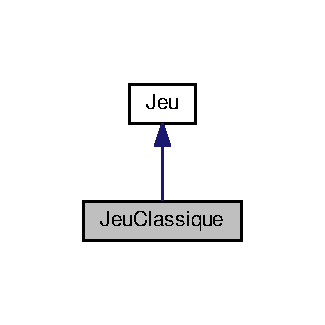
\includegraphics[width=156pt]{classJeuClassique__inherit__graph}
\end{center}
\end{figure}


Collaboration diagram for Jeu\+Classique\+:
\nopagebreak
\begin{figure}[H]
\begin{center}
\leavevmode
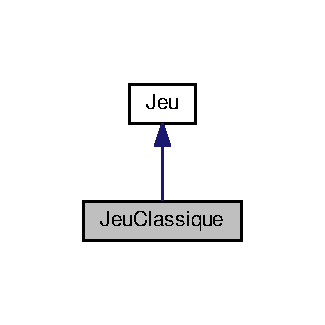
\includegraphics[width=156pt]{classJeuClassique__coll__graph}
\end{center}
\end{figure}
\subsection*{Public Member Functions}
\begin{DoxyCompactItemize}
\item 
\mbox{\Hypertarget{classJeuClassique_a9b8c0cab457b50d054746d71318be396}\label{classJeuClassique_a9b8c0cab457b50d054746d71318be396}} 
\hyperlink{classJeuClassique_a9b8c0cab457b50d054746d71318be396}{Jeu\+Classique} ()
\begin{DoxyCompactList}\small\item\em Constructeur d\textquotesingle{}un \hyperlink{classJeuClassique}{Jeu\+Classique}, c\textquotesingle{}est-\/à-\/dire d\textquotesingle{}un Tetris classique. \end{DoxyCompactList}\item 
int \hyperlink{classJeuClassique_ab6429ffc180431b667e891e329c91cb4}{getpoints} ()
\begin{DoxyCompactList}\small\item\em Accesseur du nombre de points pour un Tetris Classique. \end{DoxyCompactList}\item 
\mbox{\Hypertarget{classJeuClassique_ad61cdc881a8f6532a9bc59e91e64affb}\label{classJeuClassique_ad61cdc881a8f6532a9bc59e91e64affb}} 
void \hyperlink{classJeuClassique_ad61cdc881a8f6532a9bc59e91e64affb}{MaJ} ()
\begin{DoxyCompactList}\small\item\em Met à jour la grille après chaque action du joueur. \end{DoxyCompactList}\item 
\mbox{\Hypertarget{classJeuClassique_ab8546f30212be75a66c5735ed7fb9de4}\label{classJeuClassique_ab8546f30212be75a66c5735ed7fb9de4}} 
void \hyperlink{classJeuClassique_ab8546f30212be75a66c5735ed7fb9de4}{init} ()
\begin{DoxyCompactList}\small\item\em Initialise le jeu en début de partie. \end{DoxyCompactList}\item 
\mbox{\Hypertarget{classJeuClassique_a0d8df25a0df26319718f0c7e83b5670d}\label{classJeuClassique_a0d8df25a0df26319718f0c7e83b5670d}} 
void \hyperlink{classJeuClassique_a0d8df25a0df26319718f0c7e83b5670d}{play} ()
\begin{DoxyCompactList}\small\item\em Permet au joueur de jouer et réagit en fonction. \end{DoxyCompactList}\end{DoxyCompactItemize}


\subsection{Member Function Documentation}
\mbox{\Hypertarget{classJeuClassique_ab6429ffc180431b667e891e329c91cb4}\label{classJeuClassique_ab6429ffc180431b667e891e329c91cb4}} 
\index{Jeu\+Classique@{Jeu\+Classique}!getpoints@{getpoints}}
\index{getpoints@{getpoints}!Jeu\+Classique@{Jeu\+Classique}}
\subsubsection{\texorpdfstring{getpoints()}{getpoints()}}
{\footnotesize\ttfamily Jeu\+Classique\+::getpoints (\begin{DoxyParamCaption}{ }\end{DoxyParamCaption})}



Accesseur du nombre de points pour un Tetris Classique. 

\begin{DoxyReturn}{Returns}
le score du joueur 
\end{DoxyReturn}


The documentation for this class was generated from the following file\+:\begin{DoxyCompactItemize}
\item 
Jeu\+Classique.\+hpp\end{DoxyCompactItemize}

\hypertarget{classJeuMontagnard}{}\section{Jeu\+Montagnard Class Reference}
\label{classJeuMontagnard}\index{Jeu\+Montagnard@{Jeu\+Montagnard}}


Inheritance diagram for Jeu\+Montagnard\+:
\nopagebreak
\begin{figure}[H]
\begin{center}
\leavevmode
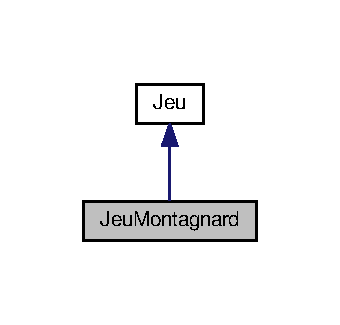
\includegraphics[width=163pt]{classJeuMontagnard__inherit__graph}
\end{center}
\end{figure}


Collaboration diagram for Jeu\+Montagnard\+:
\nopagebreak
\begin{figure}[H]
\begin{center}
\leavevmode
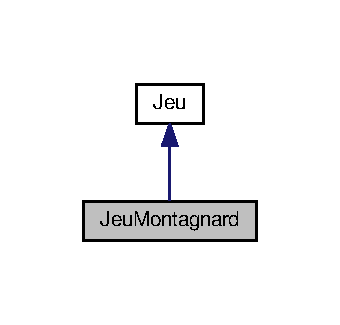
\includegraphics[width=163pt]{classJeuMontagnard__coll__graph}
\end{center}
\end{figure}
\subsection*{Public Member Functions}
\begin{DoxyCompactItemize}
\item 
\mbox{\Hypertarget{classJeuMontagnard_a8513eb021dbe504977de86eda36a0cac}\label{classJeuMontagnard_a8513eb021dbe504977de86eda36a0cac}} 
\hyperlink{classJeuMontagnard_a8513eb021dbe504977de86eda36a0cac}{Jeu\+Montagnard} ()
\begin{DoxyCompactList}\small\item\em Constructeur d\textquotesingle{}un \hyperlink{classJeuMontagnard}{Jeu\+Montagnard}, c\textquotesingle{}est-\/à-\/dire d\textquotesingle{}un Tetris avec un \hyperlink{classPersonnage}{Personnage}. \end{DoxyCompactList}\item 
int \hyperlink{classJeuMontagnard_aa4934bcc49ec59f1fd922ab6466f7a9b}{get\+Temps} ()
\begin{DoxyCompactList}\small\item\em Accesseur du temps d\textquotesingle{}une partie d\textquotesingle{}un \hyperlink{classJeuMontagnard}{Jeu\+Montagnard} pour un joueur. \end{DoxyCompactList}\item 
\mbox{\Hypertarget{classJeuMontagnard_a92ee3efc9d01dcf1ab224db9f88ff907}\label{classJeuMontagnard_a92ee3efc9d01dcf1ab224db9f88ff907}} 
void \hyperlink{classJeuMontagnard_a92ee3efc9d01dcf1ab224db9f88ff907}{MaJ} ()
\begin{DoxyCompactList}\small\item\em Met à jour la grille et le personnage après chaque action du joueur. \end{DoxyCompactList}\item 
\mbox{\Hypertarget{classJeuMontagnard_a645df2c6102b09be6cac31b94347314b}\label{classJeuMontagnard_a645df2c6102b09be6cac31b94347314b}} 
void \hyperlink{classJeuMontagnard_a645df2c6102b09be6cac31b94347314b}{init} ()
\begin{DoxyCompactList}\small\item\em Initialise le jeu et le personnage en début de partie. \end{DoxyCompactList}\item 
\mbox{\Hypertarget{classJeuMontagnard_a53262c982e4169ce371b8b49262ca7c8}\label{classJeuMontagnard_a53262c982e4169ce371b8b49262ca7c8}} 
void \hyperlink{classJeuMontagnard_a53262c982e4169ce371b8b49262ca7c8}{play} ()
\begin{DoxyCompactList}\small\item\em Permet au joueur de jouer et réagit en fonction. \end{DoxyCompactList}\end{DoxyCompactItemize}


\subsection{Member Function Documentation}
\mbox{\Hypertarget{classJeuMontagnard_aa4934bcc49ec59f1fd922ab6466f7a9b}\label{classJeuMontagnard_aa4934bcc49ec59f1fd922ab6466f7a9b}} 
\index{Jeu\+Montagnard@{Jeu\+Montagnard}!get\+Temps@{get\+Temps}}
\index{get\+Temps@{get\+Temps}!Jeu\+Montagnard@{Jeu\+Montagnard}}
\subsubsection{\texorpdfstring{get\+Temps()}{getTemps()}}
{\footnotesize\ttfamily Jeu\+Montagnard\+::get\+Temps (\begin{DoxyParamCaption}{ }\end{DoxyParamCaption})}



Accesseur du temps d\textquotesingle{}une partie d\textquotesingle{}un \hyperlink{classJeuMontagnard}{Jeu\+Montagnard} pour un joueur. 

\begin{DoxyReturn}{Returns}
le temps du joueur 
\end{DoxyReturn}


The documentation for this class was generated from the following file\+:\begin{DoxyCompactItemize}
\item 
Jeu\+Montagnard.\+hpp\end{DoxyCompactItemize}

\hypertarget{classPersonnage}{}\section{Personnage Class Reference}
\label{classPersonnage}\index{Personnage@{Personnage}}


Représentation du \hyperlink{classPersonnage}{Personnage} pour la version montagnarde du Tetris.  




{\ttfamily \#include $<$Personnage.\+hpp$>$}

\subsection*{Public Member Functions}
\begin{DoxyCompactItemize}
\item 
int \hyperlink{classPersonnage_a20df7b440cfc6f6e1b475920aa1d4215}{get\+Posx} ()
\begin{DoxyCompactList}\small\item\em Accesseur de la position en x du personnage. \end{DoxyCompactList}\item 
int \hyperlink{classPersonnage_a37c205046e1f44503e296802b66a74cd}{get\+Posy} ()
\begin{DoxyCompactList}\small\item\em Accesseur de la position en y du personnage. \end{DoxyCompactList}\item 
bool \hyperlink{classPersonnage_a4d5855ca459563583026c13072b72577}{getbloque} ()
\begin{DoxyCompactList}\small\item\em Accesseur du booléen bloqué du \hyperlink{classPersonnage}{Personnage}. \end{DoxyCompactList}\item 
bool \hyperlink{classPersonnage_a943d205f1922133e6154aabc88905ff7}{get\+Direction} ()
\begin{DoxyCompactList}\small\item\em Accesseur du booléen Direction du \hyperlink{classPersonnage}{Personnage}. \end{DoxyCompactList}\item 
void \hyperlink{classPersonnage_a3248e00e7413b2a97a7f198475318d6b}{Deplacement} (\hyperlink{classBoard}{Board} b)
\begin{DoxyCompactList}\small\item\em Permet le déplacement du \hyperlink{classPersonnage}{Personnage} dans notre grille dès que possible. \end{DoxyCompactList}\end{DoxyCompactItemize}


\subsection{Detailed Description}
Représentation du \hyperlink{classPersonnage}{Personnage} pour la version montagnarde du Tetris. 

\begin{DoxyAuthor}{Author}
Victor Le Maistre 
\end{DoxyAuthor}
\begin{DoxyVersion}{Version}
1.\+0 
\end{DoxyVersion}
\begin{DoxyDate}{Date}
avril 2018 
\end{DoxyDate}
\begin{DoxyRefDesc}{Bug}
\item[\hyperlink{bug__bug000007}{Bug}]Rien à signaler \end{DoxyRefDesc}
\begin{DoxyWarning}{Warning}
Rien à signaler
\end{DoxyWarning}
Ce module permet de représenter et d\textquotesingle{}utiliser le \hyperlink{classPersonnage}{Personnage} du Tetris montagnard. On pourra donc avoir accès à sa position en x et en y, et savoir s\textquotesingle{}il est bloqué et dans quelle direction il va 

\subsection{Member Function Documentation}
\mbox{\Hypertarget{classPersonnage_a3248e00e7413b2a97a7f198475318d6b}\label{classPersonnage_a3248e00e7413b2a97a7f198475318d6b}} 
\index{Personnage@{Personnage}!Deplacement@{Deplacement}}
\index{Deplacement@{Deplacement}!Personnage@{Personnage}}
\subsubsection{\texorpdfstring{Deplacement()}{Deplacement()}}
{\footnotesize\ttfamily void Personnage\+::\+Deplacement (\begin{DoxyParamCaption}\item[{\hyperlink{classBoard}{Board}}]{b }\end{DoxyParamCaption})}



Permet le déplacement du \hyperlink{classPersonnage}{Personnage} dans notre grille dès que possible. 


\begin{DoxyParams}{Parameters}
{\em b} & est notre grille de Tetris \\
\hline
\end{DoxyParams}
\mbox{\Hypertarget{classPersonnage_a4d5855ca459563583026c13072b72577}\label{classPersonnage_a4d5855ca459563583026c13072b72577}} 
\index{Personnage@{Personnage}!getbloque@{getbloque}}
\index{getbloque@{getbloque}!Personnage@{Personnage}}
\subsubsection{\texorpdfstring{getbloque()}{getbloque()}}
{\footnotesize\ttfamily bool Personnage\+::getbloque (\begin{DoxyParamCaption}{ }\end{DoxyParamCaption})}



Accesseur du booléen bloqué du \hyperlink{classPersonnage}{Personnage}. 

\begin{DoxyReturn}{Returns}
Retourne true si le personnage peut toujours avancer, false sinon 
\end{DoxyReturn}
\mbox{\Hypertarget{classPersonnage_a943d205f1922133e6154aabc88905ff7}\label{classPersonnage_a943d205f1922133e6154aabc88905ff7}} 
\index{Personnage@{Personnage}!get\+Direction@{get\+Direction}}
\index{get\+Direction@{get\+Direction}!Personnage@{Personnage}}
\subsubsection{\texorpdfstring{get\+Direction()}{getDirection()}}
{\footnotesize\ttfamily bool Personnage\+::get\+Direction (\begin{DoxyParamCaption}{ }\end{DoxyParamCaption})}



Accesseur du booléen Direction du \hyperlink{classPersonnage}{Personnage}. 

\begin{DoxyReturn}{Returns}
Retourne le booléen Direction 
\end{DoxyReturn}
\mbox{\Hypertarget{classPersonnage_a20df7b440cfc6f6e1b475920aa1d4215}\label{classPersonnage_a20df7b440cfc6f6e1b475920aa1d4215}} 
\index{Personnage@{Personnage}!get\+Posx@{get\+Posx}}
\index{get\+Posx@{get\+Posx}!Personnage@{Personnage}}
\subsubsection{\texorpdfstring{get\+Posx()}{getPosx()}}
{\footnotesize\ttfamily int Personnage\+::get\+Posx (\begin{DoxyParamCaption}{ }\end{DoxyParamCaption})}



Accesseur de la position en x du personnage. 

\begin{DoxyReturn}{Returns}
l\textquotesingle{}entier correspondant à la position en x du personnage dans une grille de jeu 
\end{DoxyReturn}
\mbox{\Hypertarget{classPersonnage_a37c205046e1f44503e296802b66a74cd}\label{classPersonnage_a37c205046e1f44503e296802b66a74cd}} 
\index{Personnage@{Personnage}!get\+Posy@{get\+Posy}}
\index{get\+Posy@{get\+Posy}!Personnage@{Personnage}}
\subsubsection{\texorpdfstring{get\+Posy()}{getPosy()}}
{\footnotesize\ttfamily int Personnage\+::get\+Posy (\begin{DoxyParamCaption}{ }\end{DoxyParamCaption})}



Accesseur de la position en y du personnage. 

\begin{DoxyReturn}{Returns}
l\textquotesingle{}entier correspondant à la position en y du personnage dans une grille de jeu 
\end{DoxyReturn}


The documentation for this class was generated from the following file\+:\begin{DoxyCompactItemize}
\item 
Personnage.\+hpp\end{DoxyCompactItemize}

\hypertarget{classPiece}{}\section{Piece Class Reference}
\label{classPiece}\index{Piece@{Piece}}


Représentation d\textquotesingle{}une pièce de jeu.  




{\ttfamily \#include $<$Piece.\+hpp$>$}



Inheritance diagram for Piece\+:
\nopagebreak
\begin{figure}[H]
\begin{center}
\leavevmode
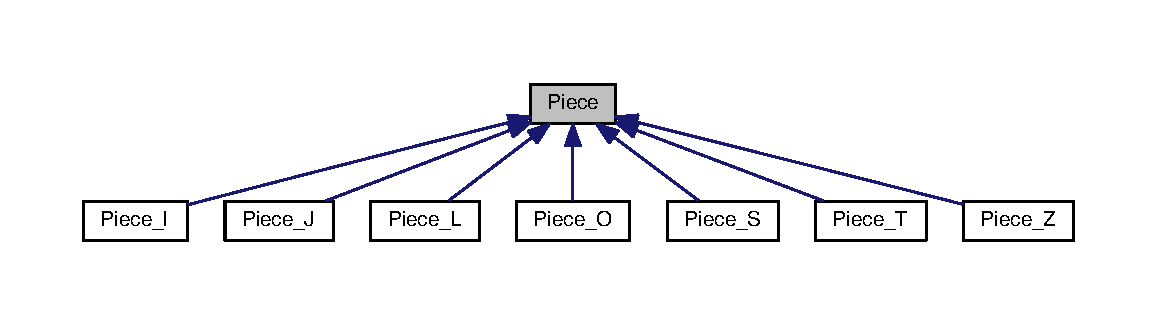
\includegraphics[width=350pt]{classPiece__inherit__graph}
\end{center}
\end{figure}
\subsection*{Public Member Functions}
\begin{DoxyCompactItemize}
\item 
int \hyperlink{classPiece_a0af5276d26a4bb2a6a42a3dab8b4783f}{get\+Posx} (int i) const
\begin{DoxyCompactList}\small\item\em Accesseur de la position en x d\textquotesingle{}un bloc. \end{DoxyCompactList}\item 
int \hyperlink{classPiece_a24ca14604d394b821bf89d690c6de477}{get\+Posy} (int i) const
\begin{DoxyCompactList}\small\item\em Accesseur de la position en y d\textquotesingle{}un bloc. \end{DoxyCompactList}\item 
void \hyperlink{classPiece_a2c6f76d78f5c448ba42b11f0b2af12f8}{set\+Posx} (int i, int j)
\begin{DoxyCompactList}\small\item\em Mutateur de la position en x d\textquotesingle{}un bloc. \end{DoxyCompactList}\item 
void \hyperlink{classPiece_a53af32e68bb73e5ed23f3ac96a9d1516}{set\+Posy} (int i, int j)
\begin{DoxyCompactList}\small\item\em Mutateur de la position en y d\textquotesingle{}un bloc. \end{DoxyCompactList}\item 
bool \hyperlink{classPiece_aa5f13b2ce17fdf29dca28b0455f7b73a}{getbloque} ()
\begin{DoxyCompactList}\small\item\em Accesseur du booléen bloqué d\textquotesingle{}une pièce. \end{DoxyCompactList}\item 
int \hyperlink{classPiece_a2160d48bd04821ebbab32e14728360ad}{getcolor} ()
\begin{DoxyCompactList}\small\item\em Accesseur de la couleur d\textquotesingle{}une pièce. \end{DoxyCompactList}\item 
bool \hyperlink{classPiece_ad48708c0bbee0b0a583f00e56808b1d2}{Down} (\hyperlink{classBoard}{Board} b)
\begin{DoxyCompactList}\small\item\em Vérifie si on peut descendre la pièce dans la grille de jeu. \end{DoxyCompactList}\item 
bool \hyperlink{classPiece_aaef48eb5277927bcacace16aaf2d9636}{Left} (\hyperlink{classBoard}{Board} b)
\begin{DoxyCompactList}\small\item\em Vérifie si on peut déplacer la pièce vers la gauche dans la grille de jeu. \end{DoxyCompactList}\item 
bool \hyperlink{classPiece_a44d684a99ea99db740b5bfa73f37ab15}{Right} (\hyperlink{classBoard}{Board} b)
\begin{DoxyCompactList}\small\item\em Vérifie si on peut déplacer la pièce vers la droite dans la grille de jeu. \end{DoxyCompactList}\item 
void \hyperlink{classPiece_a44530e200e9506f7bb4668e82dd91d54}{Move\+Down} (\hyperlink{classBoard}{Board} b)
\begin{DoxyCompactList}\small\item\em Descend la pièce d\textquotesingle{}un cran vers le bas dans la grille de jeu. \end{DoxyCompactList}\item 
void \hyperlink{classPiece_a938328bd15662dbf8d4bd66145e20e1a}{Move\+Right} (\hyperlink{classBoard}{Board} b)
\begin{DoxyCompactList}\small\item\em Décale la pièce d\textquotesingle{}un cran vers la droite dans la grille de jeu. \end{DoxyCompactList}\item 
void \hyperlink{classPiece_a08f2bd761965092bd4f8f97c81aa6af8}{Move\+Left} (\hyperlink{classBoard}{Board} b)
\begin{DoxyCompactList}\small\item\em Décale la pièce d\textquotesingle{}un cran vers le gauche dans la grille de jeu. \end{DoxyCompactList}\item 
virtual bool \hyperlink{classPiece_a56cdf7f4234fe848a3e203b693b7a862}{is\+Rotateable} (\hyperlink{classBoard}{Board} b)=0
\begin{DoxyCompactList}\small\item\em Vérifie si on peut tourner une pièce d\textquotesingle{}un cran dans le sens horaire par rapport à la grille de jeu. \end{DoxyCompactList}\item 
virtual void \hyperlink{classPiece_a078f3cc6281cb8f60af3ae2266c651ba}{Rotate} (\hyperlink{classBoard}{Board} b)=0
\begin{DoxyCompactList}\small\item\em Permet la rotation d\textquotesingle{}une pièce dans le sens horaire par rapport à la grille de jeu. \end{DoxyCompactList}\item 
\mbox{\Hypertarget{classPiece_ac57de5803bbad829b143bc7268267dc1}\label{classPiece_ac57de5803bbad829b143bc7268267dc1}} 
\hyperlink{classPiece_ac57de5803bbad829b143bc7268267dc1}{Piece} ()
\begin{DoxyCompactList}\small\item\em Constructeur d\textquotesingle{}une piece de jeu général. \end{DoxyCompactList}\end{DoxyCompactItemize}
\subsection*{Protected Attributes}
\begin{DoxyCompactItemize}
\item 
vector$<$ \hyperlink{classBloc}{Bloc} $>$ \hyperlink{classPiece_a9ea65e906b9ef0c30594f4f5aa5ed444}{tab}
\item 
int \hyperlink{classPiece_a9632e25aa0e79f8161451a937ccfc7ad}{etat}
\item 
bool \hyperlink{classPiece_a99b4e2bbf91e0e609fc5141135a2e0ad}{bloque}
\item 
int \hyperlink{classPiece_a4268f3b047e1ad284882708b85332ef1}{color}
\item 
bool \hyperlink{classPiece_af0c815c20f2000c02b6d7ce5b6703651}{stocke}
\end{DoxyCompactItemize}


\subsection{Detailed Description}
Représentation d\textquotesingle{}une pièce de jeu. 

\begin{DoxyAuthor}{Author}
Léa Lefrançois 

Laura Couret 

Victor Le Maistre 
\end{DoxyAuthor}
\begin{DoxyVersion}{Version}
1.\+0 
\end{DoxyVersion}
\begin{DoxyDate}{Date}
avril 2018 
\end{DoxyDate}
\begin{DoxyRefDesc}{Bug}
\item[\hyperlink{bug__bug000008}{Bug}]Rien à signaler \end{DoxyRefDesc}
\begin{DoxyWarning}{Warning}
Rien à signaler
\end{DoxyWarning}
Ce module permet la représentation physique d\textquotesingle{}une pièce par sa position, son état et sa couleur. Plus particulièrement, on pourra changer les paramètres caractéristiques de la pièce, vérifier si on peut la déplacer ou la tourner, la déplacer dans les 3 sens (gauche, droite, bas), et la tourner dans le sens horaire ou dans le sens trigonométrique. 

\subsection{Member Function Documentation}
\mbox{\Hypertarget{classPiece_ad48708c0bbee0b0a583f00e56808b1d2}\label{classPiece_ad48708c0bbee0b0a583f00e56808b1d2}} 
\index{Piece@{Piece}!Down@{Down}}
\index{Down@{Down}!Piece@{Piece}}
\subsubsection{\texorpdfstring{Down()}{Down()}}
{\footnotesize\ttfamily bool Piece\+::\+Down (\begin{DoxyParamCaption}\item[{\hyperlink{classBoard}{Board}}]{b }\end{DoxyParamCaption})}



Vérifie si on peut descendre la pièce dans la grille de jeu. 


\begin{DoxyParams}{Parameters}
{\em b} & est la grille de notre Tetris \\
\hline
\end{DoxyParams}
\begin{DoxyReturn}{Returns}
true si on peut descendre la pièce d\textquotesingle{}un cran, false sinon 
\end{DoxyReturn}
\mbox{\Hypertarget{classPiece_aa5f13b2ce17fdf29dca28b0455f7b73a}\label{classPiece_aa5f13b2ce17fdf29dca28b0455f7b73a}} 
\index{Piece@{Piece}!getbloque@{getbloque}}
\index{getbloque@{getbloque}!Piece@{Piece}}
\subsubsection{\texorpdfstring{getbloque()}{getbloque()}}
{\footnotesize\ttfamily bool Piece\+::getbloque (\begin{DoxyParamCaption}{ }\end{DoxyParamCaption})}



Accesseur du booléen bloqué d\textquotesingle{}une pièce. 

\begin{DoxyReturn}{Returns}
Retourne le booléen bloque 
\end{DoxyReturn}
\mbox{\Hypertarget{classPiece_a2160d48bd04821ebbab32e14728360ad}\label{classPiece_a2160d48bd04821ebbab32e14728360ad}} 
\index{Piece@{Piece}!getcolor@{getcolor}}
\index{getcolor@{getcolor}!Piece@{Piece}}
\subsubsection{\texorpdfstring{getcolor()}{getcolor()}}
{\footnotesize\ttfamily int Piece\+::getcolor (\begin{DoxyParamCaption}{ }\end{DoxyParamCaption})}



Accesseur de la couleur d\textquotesingle{}une pièce. 

\begin{DoxyReturn}{Returns}
Retourne l\textquotesingle{}entier correspondant à la couleur de la pièce 
\end{DoxyReturn}
\mbox{\Hypertarget{classPiece_a0af5276d26a4bb2a6a42a3dab8b4783f}\label{classPiece_a0af5276d26a4bb2a6a42a3dab8b4783f}} 
\index{Piece@{Piece}!get\+Posx@{get\+Posx}}
\index{get\+Posx@{get\+Posx}!Piece@{Piece}}
\subsubsection{\texorpdfstring{get\+Posx()}{getPosx()}}
{\footnotesize\ttfamily int Piece\+::get\+Posx (\begin{DoxyParamCaption}\item[{int}]{i }\end{DoxyParamCaption}) const}



Accesseur de la position en x d\textquotesingle{}un bloc. 


\begin{DoxyParams}{Parameters}
{\em i} & est le numéro du bloc dont on veut obtenir les informations \\
\hline
\end{DoxyParams}
\begin{DoxyReturn}{Returns}
Retourne la position en x du bloc numero i de la pièce en question 
\end{DoxyReturn}
\mbox{\Hypertarget{classPiece_a24ca14604d394b821bf89d690c6de477}\label{classPiece_a24ca14604d394b821bf89d690c6de477}} 
\index{Piece@{Piece}!get\+Posy@{get\+Posy}}
\index{get\+Posy@{get\+Posy}!Piece@{Piece}}
\subsubsection{\texorpdfstring{get\+Posy()}{getPosy()}}
{\footnotesize\ttfamily int Piece\+::get\+Posy (\begin{DoxyParamCaption}\item[{int}]{i }\end{DoxyParamCaption}) const}



Accesseur de la position en y d\textquotesingle{}un bloc. 


\begin{DoxyParams}{Parameters}
{\em i} & est le numéro du bloc dont on veut obtenir les informations \\
\hline
\end{DoxyParams}
\begin{DoxyReturn}{Returns}
Retourne la position en y du bloc numero i de la pièce en question 
\end{DoxyReturn}
\mbox{\Hypertarget{classPiece_a56cdf7f4234fe848a3e203b693b7a862}\label{classPiece_a56cdf7f4234fe848a3e203b693b7a862}} 
\index{Piece@{Piece}!is\+Rotateable@{is\+Rotateable}}
\index{is\+Rotateable@{is\+Rotateable}!Piece@{Piece}}
\subsubsection{\texorpdfstring{is\+Rotateable()}{isRotateable()}}
{\footnotesize\ttfamily bool Piece\+::is\+Rotateable (\begin{DoxyParamCaption}\item[{\hyperlink{classBoard}{Board}}]{b }\end{DoxyParamCaption})\hspace{0.3cm}{\ttfamily [pure virtual]}}



Vérifie si on peut tourner une pièce d\textquotesingle{}un cran dans le sens horaire par rapport à la grille de jeu. 


\begin{DoxyParams}{Parameters}
{\em b} & est la grille de notre Tetris \\
\hline
\end{DoxyParams}


Implemented in \hyperlink{classPiece__O_af82900ecec4e7bd058d43825293d8bff}{Piece\+\_\+O}, \hyperlink{classPiece__I_aec103ce64d2702bf3dc5dbcdb8b450eb}{Piece\+\_\+I}, \hyperlink{classPiece__T_a64088f0140b870d178169e36460cd4de}{Piece\+\_\+T}, \hyperlink{classPiece__J_aee0abd6254be3a50a86ff5464bb459f8}{Piece\+\_\+J}, \hyperlink{classPiece__L_a34954ce32a27bdadb4d56ca7f3d82cba}{Piece\+\_\+L}, \hyperlink{classPiece__S_a725b9e7b154628e035bcc7ebd2a3ec9f}{Piece\+\_\+S}, and \hyperlink{classPiece__Z_aa70256d6f49dacad685a15c5ae8df06d}{Piece\+\_\+Z}.

\mbox{\Hypertarget{classPiece_aaef48eb5277927bcacace16aaf2d9636}\label{classPiece_aaef48eb5277927bcacace16aaf2d9636}} 
\index{Piece@{Piece}!Left@{Left}}
\index{Left@{Left}!Piece@{Piece}}
\subsubsection{\texorpdfstring{Left()}{Left()}}
{\footnotesize\ttfamily bool Piece\+::\+Left (\begin{DoxyParamCaption}\item[{\hyperlink{classBoard}{Board}}]{b }\end{DoxyParamCaption})}



Vérifie si on peut déplacer la pièce vers la gauche dans la grille de jeu. 


\begin{DoxyParams}{Parameters}
{\em b} & est la grille de notre Tetris \\
\hline
\end{DoxyParams}
\begin{DoxyReturn}{Returns}
true si on peut déplacer la pièce d\textquotesingle{}un cran vers la gauche, false sinon 
\end{DoxyReturn}
\mbox{\Hypertarget{classPiece_a44530e200e9506f7bb4668e82dd91d54}\label{classPiece_a44530e200e9506f7bb4668e82dd91d54}} 
\index{Piece@{Piece}!Move\+Down@{Move\+Down}}
\index{Move\+Down@{Move\+Down}!Piece@{Piece}}
\subsubsection{\texorpdfstring{Move\+Down()}{MoveDown()}}
{\footnotesize\ttfamily void Piece\+::\+Move\+Down (\begin{DoxyParamCaption}\item[{\hyperlink{classBoard}{Board}}]{b }\end{DoxyParamCaption})}



Descend la pièce d\textquotesingle{}un cran vers le bas dans la grille de jeu. 


\begin{DoxyParams}{Parameters}
{\em b} & est la grille de notre Tetris \\
\hline
\end{DoxyParams}
\mbox{\Hypertarget{classPiece_a08f2bd761965092bd4f8f97c81aa6af8}\label{classPiece_a08f2bd761965092bd4f8f97c81aa6af8}} 
\index{Piece@{Piece}!Move\+Left@{Move\+Left}}
\index{Move\+Left@{Move\+Left}!Piece@{Piece}}
\subsubsection{\texorpdfstring{Move\+Left()}{MoveLeft()}}
{\footnotesize\ttfamily void Piece\+::\+Move\+Left (\begin{DoxyParamCaption}\item[{\hyperlink{classBoard}{Board}}]{b }\end{DoxyParamCaption})}



Décale la pièce d\textquotesingle{}un cran vers le gauche dans la grille de jeu. 


\begin{DoxyParams}{Parameters}
{\em b} & est la grille de notre Tetris \\
\hline
\end{DoxyParams}
\mbox{\Hypertarget{classPiece_a938328bd15662dbf8d4bd66145e20e1a}\label{classPiece_a938328bd15662dbf8d4bd66145e20e1a}} 
\index{Piece@{Piece}!Move\+Right@{Move\+Right}}
\index{Move\+Right@{Move\+Right}!Piece@{Piece}}
\subsubsection{\texorpdfstring{Move\+Right()}{MoveRight()}}
{\footnotesize\ttfamily void Piece\+::\+Move\+Right (\begin{DoxyParamCaption}\item[{\hyperlink{classBoard}{Board}}]{b }\end{DoxyParamCaption})}



Décale la pièce d\textquotesingle{}un cran vers la droite dans la grille de jeu. 


\begin{DoxyParams}{Parameters}
{\em b} & est la grille de notre Tetris \\
\hline
\end{DoxyParams}
\mbox{\Hypertarget{classPiece_a44d684a99ea99db740b5bfa73f37ab15}\label{classPiece_a44d684a99ea99db740b5bfa73f37ab15}} 
\index{Piece@{Piece}!Right@{Right}}
\index{Right@{Right}!Piece@{Piece}}
\subsubsection{\texorpdfstring{Right()}{Right()}}
{\footnotesize\ttfamily bool Piece\+::\+Right (\begin{DoxyParamCaption}\item[{\hyperlink{classBoard}{Board}}]{b }\end{DoxyParamCaption})}



Vérifie si on peut déplacer la pièce vers la droite dans la grille de jeu. 


\begin{DoxyParams}{Parameters}
{\em b} & est la grille de notre Tetris \\
\hline
\end{DoxyParams}
\begin{DoxyReturn}{Returns}
true si on peut déplacer la pièce d\textquotesingle{}un cran vers la droite, false sinon 
\end{DoxyReturn}
\mbox{\Hypertarget{classPiece_a078f3cc6281cb8f60af3ae2266c651ba}\label{classPiece_a078f3cc6281cb8f60af3ae2266c651ba}} 
\index{Piece@{Piece}!Rotate@{Rotate}}
\index{Rotate@{Rotate}!Piece@{Piece}}
\subsubsection{\texorpdfstring{Rotate()}{Rotate()}}
{\footnotesize\ttfamily void Piece\+::\+Rotate (\begin{DoxyParamCaption}\item[{\hyperlink{classBoard}{Board}}]{b }\end{DoxyParamCaption})\hspace{0.3cm}{\ttfamily [pure virtual]}}



Permet la rotation d\textquotesingle{}une pièce dans le sens horaire par rapport à la grille de jeu. 


\begin{DoxyParams}{Parameters}
{\em b} & est la grille de notre Tetris \\
\hline
\end{DoxyParams}


Implemented in \hyperlink{classPiece__O_a69812f938582f176cd4cca997cbb87c1}{Piece\+\_\+O}, \hyperlink{classPiece__I_ab7983a575f6d5d41cbf846b6240a9b43}{Piece\+\_\+I}, \hyperlink{classPiece__T_affedcbe550aebd2a9e8ec169d1fe0a9f}{Piece\+\_\+T}, \hyperlink{classPiece__J_a05b85a353b6d5cefb0055206d4a39014}{Piece\+\_\+J}, \hyperlink{classPiece__L_aa865e9d2c6c468ac2921d6adb88f4d1b}{Piece\+\_\+L}, \hyperlink{classPiece__S_aefb2837f39f6b05bc678a3fdadc192b0}{Piece\+\_\+S}, and \hyperlink{classPiece__Z_a50d6c34030c7641b4827353b9b82a68e}{Piece\+\_\+Z}.

\mbox{\Hypertarget{classPiece_a2c6f76d78f5c448ba42b11f0b2af12f8}\label{classPiece_a2c6f76d78f5c448ba42b11f0b2af12f8}} 
\index{Piece@{Piece}!set\+Posx@{set\+Posx}}
\index{set\+Posx@{set\+Posx}!Piece@{Piece}}
\subsubsection{\texorpdfstring{set\+Posx()}{setPosx()}}
{\footnotesize\ttfamily int Piece\+::set\+Posx (\begin{DoxyParamCaption}\item[{int}]{i,  }\item[{int}]{j }\end{DoxyParamCaption})}



Mutateur de la position en x d\textquotesingle{}un bloc. 


\begin{DoxyParams}{Parameters}
{\em i} & est le numéro du bloc dont on veut modifier la position en x par j \\
\hline
\end{DoxyParams}
\mbox{\Hypertarget{classPiece_a53af32e68bb73e5ed23f3ac96a9d1516}\label{classPiece_a53af32e68bb73e5ed23f3ac96a9d1516}} 
\index{Piece@{Piece}!set\+Posy@{set\+Posy}}
\index{set\+Posy@{set\+Posy}!Piece@{Piece}}
\subsubsection{\texorpdfstring{set\+Posy()}{setPosy()}}
{\footnotesize\ttfamily int Piece\+::set\+Posy (\begin{DoxyParamCaption}\item[{int}]{i,  }\item[{int}]{j }\end{DoxyParamCaption})}



Mutateur de la position en y d\textquotesingle{}un bloc. 


\begin{DoxyParams}{Parameters}
{\em i} & est le numéro du bloc dont on veut modifier la position en y par j \\
\hline
\end{DoxyParams}


\subsection{Member Data Documentation}
\mbox{\Hypertarget{classPiece_a99b4e2bbf91e0e609fc5141135a2e0ad}\label{classPiece_a99b4e2bbf91e0e609fc5141135a2e0ad}} 
\index{Piece@{Piece}!bloque@{bloque}}
\index{bloque@{bloque}!Piece@{Piece}}
\subsubsection{\texorpdfstring{bloque}{bloque}}
{\footnotesize\ttfamily bool Piece\+::bloque\hspace{0.3cm}{\ttfamily [protected]}}

/var bloque est un booleen qui permet de savoir si une pièce a atteint sa position finale dans la grille de jeu ou si elle peut encore descendre \mbox{\Hypertarget{classPiece_a4268f3b047e1ad284882708b85332ef1}\label{classPiece_a4268f3b047e1ad284882708b85332ef1}} 
\index{Piece@{Piece}!color@{color}}
\index{color@{color}!Piece@{Piece}}
\subsubsection{\texorpdfstring{color}{color}}
{\footnotesize\ttfamily int Piece\+::color\hspace{0.3cm}{\ttfamily [protected]}}

/var color définit la couleur de la piece \mbox{\Hypertarget{classPiece_a9632e25aa0e79f8161451a937ccfc7ad}\label{classPiece_a9632e25aa0e79f8161451a937ccfc7ad}} 
\index{Piece@{Piece}!etat@{etat}}
\index{etat@{etat}!Piece@{Piece}}
\subsubsection{\texorpdfstring{etat}{etat}}
{\footnotesize\ttfamily int Piece\+::etat\hspace{0.3cm}{\ttfamily [protected]}}

/var etat correspond à dans quel état de rotation se situe la pièce \mbox{\Hypertarget{classPiece_af0c815c20f2000c02b6d7ce5b6703651}\label{classPiece_af0c815c20f2000c02b6d7ce5b6703651}} 
\index{Piece@{Piece}!stocke@{stocke}}
\index{stocke@{stocke}!Piece@{Piece}}
\subsubsection{\texorpdfstring{stocke}{stocke}}
{\footnotesize\ttfamily bool Piece\+::stocke\hspace{0.3cm}{\ttfamily [protected]}}

/var stocke permet de savoir si une pièce peut être stocké. Attention, une pièce ne peut être stockée qu\textquotesingle{}une fois. \mbox{\Hypertarget{classPiece_a9ea65e906b9ef0c30594f4f5aa5ed444}\label{classPiece_a9ea65e906b9ef0c30594f4f5aa5ed444}} 
\index{Piece@{Piece}!tab@{tab}}
\index{tab@{tab}!Piece@{Piece}}
\subsubsection{\texorpdfstring{tab}{tab}}
{\footnotesize\ttfamily vector$<$\hyperlink{classBloc}{Bloc}$>$ Piece\+::tab\hspace{0.3cm}{\ttfamily [protected]}}

/var tab un vecteur de \hyperlink{classBloc}{Bloc}, c\textquotesingle{}est-\/à-\/dire un vecteur où chaque case a pour attribut la position en x et la position en y 

The documentation for this class was generated from the following files\+:\begin{DoxyCompactItemize}
\item 
Piece.\+hpp\item 
Piece.\+cpp\end{DoxyCompactItemize}

\hypertarget{classPiece__I}{}\section{Piece\+\_\+I Class Reference}
\label{classPiece__I}\index{Piece\+\_\+I@{Piece\+\_\+I}}


Représentation d\textquotesingle{}un Tétrimino en forme de I. Hérite de \hyperlink{classPiece}{Piece}.  




{\ttfamily \#include $<$Piece\+\_\+\+I.\+hpp$>$}



Inheritance diagram for Piece\+\_\+I\+:
\nopagebreak
\begin{figure}[H]
\begin{center}
\leavevmode
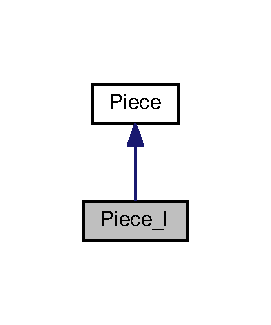
\includegraphics[width=130pt]{classPiece__I__inherit__graph}
\end{center}
\end{figure}


Collaboration diagram for Piece\+\_\+I\+:
\nopagebreak
\begin{figure}[H]
\begin{center}
\leavevmode
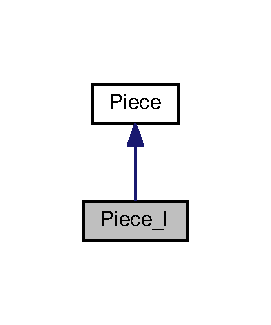
\includegraphics[width=130pt]{classPiece__I__coll__graph}
\end{center}
\end{figure}
\subsection*{Public Member Functions}
\begin{DoxyCompactItemize}
\item 
virtual bool \hyperlink{classPiece__I_aec103ce64d2702bf3dc5dbcdb8b450eb}{is\+Rotateable} (\hyperlink{classBoard}{Board} b)
\begin{DoxyCompactList}\small\item\em Vérifie si on peut tourner le Tétrimino en forme de I d\textquotesingle{}un cran dans le sens horaire par rapport au \hyperlink{classBoard}{Board}. \end{DoxyCompactList}\item 
virtual void \hyperlink{classPiece__I_ab7983a575f6d5d41cbf846b6240a9b43}{Rotate} (\hyperlink{classBoard}{Board} b)
\begin{DoxyCompactList}\small\item\em Permet la rotation d\textquotesingle{}un Tétrimino en forme de I dans le sens horaire par rapport au \hyperlink{classBoard}{Board}. \end{DoxyCompactList}\item 
\mbox{\Hypertarget{classPiece__I_a02fe6ccd07ebfbf22ce8ee6edcdd118e}\label{classPiece__I_a02fe6ccd07ebfbf22ce8ee6edcdd118e}} 
\hyperlink{classPiece__I_a02fe6ccd07ebfbf22ce8ee6edcdd118e}{Piece\+\_\+I} ()
\begin{DoxyCompactList}\small\item\em constructeur qui permet la création d\textquotesingle{}un Tétrimino en forme de I, composé de 4 cases. A son initilisation, il est en position verticale. \end{DoxyCompactList}\end{DoxyCompactItemize}
\subsection*{Additional Inherited Members}


\subsection{Detailed Description}
Représentation d\textquotesingle{}un Tétrimino en forme de I. Hérite de \hyperlink{classPiece}{Piece}. 

\begin{DoxyAuthor}{Author}
Léa Lefrançois 

Laura Couret 
\end{DoxyAuthor}
\begin{DoxyVersion}{Version}
1.\+0 
\end{DoxyVersion}
\begin{DoxyDate}{Date}
avril 2018 
\end{DoxyDate}
\begin{DoxyRefDesc}{Bug}
\item[\hyperlink{bug__bug000011}{Bug}]Rien à signaler \end{DoxyRefDesc}
\begin{DoxyWarning}{Warning}
Rien à signaler
\end{DoxyWarning}
Ce module permet la représentation physique d\textquotesingle{}un Tétrimino en forme de I. Cette classe hérite de \hyperlink{classPiece}{Piece}, elle hérite donc de ses paramètres (couleur, etat, position, etc) et gardera ses méthodes de déplacement. 

\subsection{Member Function Documentation}
\mbox{\Hypertarget{classPiece__I_aec103ce64d2702bf3dc5dbcdb8b450eb}\label{classPiece__I_aec103ce64d2702bf3dc5dbcdb8b450eb}} 
\index{Piece\+\_\+I@{Piece\+\_\+I}!is\+Rotateable@{is\+Rotateable}}
\index{is\+Rotateable@{is\+Rotateable}!Piece\+\_\+I@{Piece\+\_\+I}}
\subsubsection{\texorpdfstring{is\+Rotateable()}{isRotateable()}}
{\footnotesize\ttfamily bool Piece\+\_\+\+I\+::is\+Rotateable (\begin{DoxyParamCaption}\item[{\hyperlink{classBoard}{Board}}]{b }\end{DoxyParamCaption})\hspace{0.3cm}{\ttfamily [virtual]}}



Vérifie si on peut tourner le Tétrimino en forme de I d\textquotesingle{}un cran dans le sens horaire par rapport au \hyperlink{classBoard}{Board}. 


\begin{DoxyParams}{Parameters}
{\em b} & est le \hyperlink{classBoard}{Board} de notre Tetris \\
\hline
\end{DoxyParams}


Implements \hyperlink{classPiece_a56cdf7f4234fe848a3e203b693b7a862}{Piece}.

\mbox{\Hypertarget{classPiece__I_ab7983a575f6d5d41cbf846b6240a9b43}\label{classPiece__I_ab7983a575f6d5d41cbf846b6240a9b43}} 
\index{Piece\+\_\+I@{Piece\+\_\+I}!Rotate@{Rotate}}
\index{Rotate@{Rotate}!Piece\+\_\+I@{Piece\+\_\+I}}
\subsubsection{\texorpdfstring{Rotate()}{Rotate()}}
{\footnotesize\ttfamily void Piece\+\_\+\+I\+::\+Rotate (\begin{DoxyParamCaption}\item[{\hyperlink{classBoard}{Board}}]{b }\end{DoxyParamCaption})\hspace{0.3cm}{\ttfamily [virtual]}}



Permet la rotation d\textquotesingle{}un Tétrimino en forme de I dans le sens horaire par rapport au \hyperlink{classBoard}{Board}. 


\begin{DoxyParams}{Parameters}
{\em b} & est le \hyperlink{classBoard}{Board} de notre Tetris \\
\hline
\end{DoxyParams}


Implements \hyperlink{classPiece_a078f3cc6281cb8f60af3ae2266c651ba}{Piece}.



The documentation for this class was generated from the following files\+:\begin{DoxyCompactItemize}
\item 
Piece\+\_\+\+I.\+hpp\item 
Piece\+\_\+\+I.\+cpp\end{DoxyCompactItemize}

\hypertarget{classPiece__J}{}\section{Piece\+\_\+J Class Reference}
\label{classPiece__J}\index{Piece\+\_\+J@{Piece\+\_\+J}}


Représentation d\textquotesingle{}un Tétrimino en forme de J. Hérite de Pièce.  




{\ttfamily \#include $<$Piece\+\_\+\+J.\+hpp$>$}



Inheritance diagram for Piece\+\_\+J\+:
\nopagebreak
\begin{figure}[H]
\begin{center}
\leavevmode
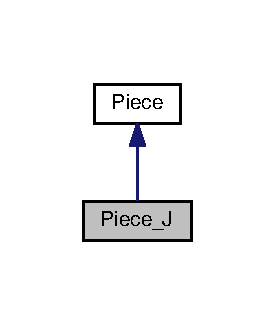
\includegraphics[width=132pt]{classPiece__J__inherit__graph}
\end{center}
\end{figure}


Collaboration diagram for Piece\+\_\+J\+:
\nopagebreak
\begin{figure}[H]
\begin{center}
\leavevmode
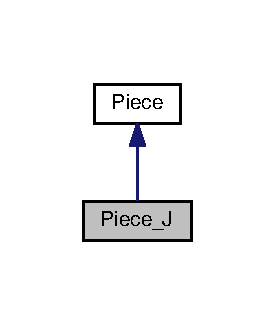
\includegraphics[width=132pt]{classPiece__J__coll__graph}
\end{center}
\end{figure}
\subsection*{Public Member Functions}
\begin{DoxyCompactItemize}
\item 
bool \hyperlink{classPiece__J_aee0abd6254be3a50a86ff5464bb459f8}{is\+Rotateable} (\hyperlink{classBoard}{Board} b)
\begin{DoxyCompactList}\small\item\em Vérifie si on peut tourner le Tétrimino en forme de J d\textquotesingle{}un cran dans le sens horaire par rapport à la grille de jeu. \end{DoxyCompactList}\item 
void \hyperlink{classPiece__J_a05b85a353b6d5cefb0055206d4a39014}{Rotate} (\hyperlink{classBoard}{Board} b)
\begin{DoxyCompactList}\small\item\em Permet la rotation d\textquotesingle{}un Tétrimino en forme de J dans le sens horaire par rapport à la grille de jeu. \end{DoxyCompactList}\item 
\mbox{\Hypertarget{classPiece__J_ac7299340d86be483ba59e3befce76327}\label{classPiece__J_ac7299340d86be483ba59e3befce76327}} 
\hyperlink{classPiece__J_ac7299340d86be483ba59e3befce76327}{Piece\+\_\+J} ()
\begin{DoxyCompactList}\small\item\em constructeur qui permet la création d\textquotesingle{}un Tétrimino en forme de J, composé de 4 cases. A son initilisation, il est en position \+: 3 cases en ligne et une case sous le côté droit. \end{DoxyCompactList}\end{DoxyCompactItemize}
\subsection*{Additional Inherited Members}


\subsection{Detailed Description}
Représentation d\textquotesingle{}un Tétrimino en forme de J. Hérite de Pièce. 

\begin{DoxyAuthor}{Author}
Laura Couret 
\end{DoxyAuthor}
\begin{DoxyVersion}{Version}
1.\+0 
\end{DoxyVersion}
\begin{DoxyDate}{Date}
avril 2018 
\end{DoxyDate}
\begin{DoxyRefDesc}{Bug}
\item[\hyperlink{bug__bug000010}{Bug}]Rien à signaler \end{DoxyRefDesc}
\begin{DoxyWarning}{Warning}
Rien à signaler
\end{DoxyWarning}
Ce module permet la représentation physique d\textquotesingle{}un Tétrimino en forme de J. Cette classe hérite de Pièce, elle hérite donc de ses paramètres (couleur, etat, position, etc) et gardera ses méthodes de déplacement. 

\subsection{Member Function Documentation}
\mbox{\Hypertarget{classPiece__J_aee0abd6254be3a50a86ff5464bb459f8}\label{classPiece__J_aee0abd6254be3a50a86ff5464bb459f8}} 
\index{Piece\+\_\+J@{Piece\+\_\+J}!is\+Rotateable@{is\+Rotateable}}
\index{is\+Rotateable@{is\+Rotateable}!Piece\+\_\+J@{Piece\+\_\+J}}
\subsubsection{\texorpdfstring{is\+Rotateable()}{isRotateable()}}
{\footnotesize\ttfamily bool Piece\+\_\+\+J\+::is\+Rotateable (\begin{DoxyParamCaption}\item[{\hyperlink{classBoard}{Board}}]{b }\end{DoxyParamCaption})\hspace{0.3cm}{\ttfamily [virtual]}}



Vérifie si on peut tourner le Tétrimino en forme de J d\textquotesingle{}un cran dans le sens horaire par rapport à la grille de jeu. 


\begin{DoxyParams}{Parameters}
{\em b} & est la grille de notre Tetris \\
\hline
\end{DoxyParams}


Implements \hyperlink{classPiece_a56cdf7f4234fe848a3e203b693b7a862}{Piece}.

\mbox{\Hypertarget{classPiece__J_a05b85a353b6d5cefb0055206d4a39014}\label{classPiece__J_a05b85a353b6d5cefb0055206d4a39014}} 
\index{Piece\+\_\+J@{Piece\+\_\+J}!Rotate@{Rotate}}
\index{Rotate@{Rotate}!Piece\+\_\+J@{Piece\+\_\+J}}
\subsubsection{\texorpdfstring{Rotate()}{Rotate()}}
{\footnotesize\ttfamily void Piece\+\_\+\+J\+::\+Rotate (\begin{DoxyParamCaption}\item[{\hyperlink{classBoard}{Board}}]{b }\end{DoxyParamCaption})\hspace{0.3cm}{\ttfamily [virtual]}}



Permet la rotation d\textquotesingle{}un Tétrimino en forme de J dans le sens horaire par rapport à la grille de jeu. 


\begin{DoxyParams}{Parameters}
{\em b} & est la grille de notre Tetris \\
\hline
\end{DoxyParams}


Implements \hyperlink{classPiece_a078f3cc6281cb8f60af3ae2266c651ba}{Piece}.



The documentation for this class was generated from the following files\+:\begin{DoxyCompactItemize}
\item 
Piece\+\_\+\+J.\+hpp\item 
Piece\+\_\+\+J.\+cpp\end{DoxyCompactItemize}

\hypertarget{classPiece__L}{}\section{Piece\+\_\+L Class Reference}
\label{classPiece__L}\index{Piece\+\_\+L@{Piece\+\_\+L}}


Représentation d\textquotesingle{}un Tétrimino en forme de L. Hérite de \hyperlink{classPiece}{Piece}.  




{\ttfamily \#include $<$Piece\+\_\+\+L.\+hpp$>$}



Inheritance diagram for Piece\+\_\+L\+:
\nopagebreak
\begin{figure}[H]
\begin{center}
\leavevmode
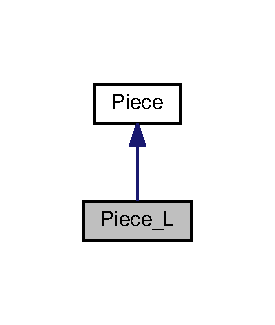
\includegraphics[width=132pt]{classPiece__L__inherit__graph}
\end{center}
\end{figure}


Collaboration diagram for Piece\+\_\+L\+:
\nopagebreak
\begin{figure}[H]
\begin{center}
\leavevmode
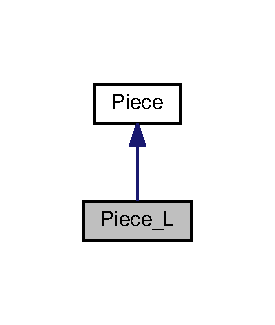
\includegraphics[width=132pt]{classPiece__L__coll__graph}
\end{center}
\end{figure}
\subsection*{Public Member Functions}
\begin{DoxyCompactItemize}
\item 
bool \hyperlink{classPiece__L_a34954ce32a27bdadb4d56ca7f3d82cba}{is\+Rotateable} (\hyperlink{classBoard}{Board} b)
\begin{DoxyCompactList}\small\item\em Vérifie si on peut tourner le Tétrimino en forme de L d\textquotesingle{}un cran dans le sens horaire par rapport au \hyperlink{classBoard}{Board}. \end{DoxyCompactList}\item 
void \hyperlink{classPiece__L_aa865e9d2c6c468ac2921d6adb88f4d1b}{Rotate} (\hyperlink{classBoard}{Board} b)
\begin{DoxyCompactList}\small\item\em Permet la rotation d\textquotesingle{}un Tétrimino en forme de L dans le sens horaire par rapport au \hyperlink{classBoard}{Board}. \end{DoxyCompactList}\item 
\mbox{\Hypertarget{classPiece__L_a2cd2017561857128dfc8838fc90e3e0b}\label{classPiece__L_a2cd2017561857128dfc8838fc90e3e0b}} 
\hyperlink{classPiece__L_a2cd2017561857128dfc8838fc90e3e0b}{Piece\+\_\+L} ()
\begin{DoxyCompactList}\small\item\em constructeur qui permet la création d\textquotesingle{}un Tétrimino en forme de L, composé de 4 cases. A son initilisation, il est en position \+: 3 cases en ligne et une case sous le côté gauche. \end{DoxyCompactList}\end{DoxyCompactItemize}
\subsection*{Additional Inherited Members}


\subsection{Detailed Description}
Représentation d\textquotesingle{}un Tétrimino en forme de L. Hérite de \hyperlink{classPiece}{Piece}. 

\begin{DoxyAuthor}{Author}
Laura Couret 
\end{DoxyAuthor}
\begin{DoxyVersion}{Version}
1.\+0 
\end{DoxyVersion}
\begin{DoxyDate}{Date}
avril 2018 
\end{DoxyDate}
\begin{DoxyRefDesc}{Bug}
\item[\hyperlink{bug__bug000013}{Bug}]Rien à signaler \end{DoxyRefDesc}
\begin{DoxyWarning}{Warning}
Rien à signaler
\end{DoxyWarning}
Ce module permet la représentation physique d\textquotesingle{}un Tétrimino en forme de L. Cette classe hérite de \hyperlink{classPiece}{Piece}, elle hérite donc de ses paramètres (couleur, etat, position, etc) et gardera ses méthodes de déplacement. 

\subsection{Member Function Documentation}
\mbox{\Hypertarget{classPiece__L_a34954ce32a27bdadb4d56ca7f3d82cba}\label{classPiece__L_a34954ce32a27bdadb4d56ca7f3d82cba}} 
\index{Piece\+\_\+L@{Piece\+\_\+L}!is\+Rotateable@{is\+Rotateable}}
\index{is\+Rotateable@{is\+Rotateable}!Piece\+\_\+L@{Piece\+\_\+L}}
\subsubsection{\texorpdfstring{is\+Rotateable()}{isRotateable()}}
{\footnotesize\ttfamily bool Piece\+\_\+\+L\+::is\+Rotateable (\begin{DoxyParamCaption}\item[{\hyperlink{classBoard}{Board}}]{b }\end{DoxyParamCaption})\hspace{0.3cm}{\ttfamily [virtual]}}



Vérifie si on peut tourner le Tétrimino en forme de L d\textquotesingle{}un cran dans le sens horaire par rapport au \hyperlink{classBoard}{Board}. 


\begin{DoxyParams}{Parameters}
{\em b} & est le \hyperlink{classBoard}{Board} de notre Tetris \\
\hline
\end{DoxyParams}


Implements \hyperlink{classPiece_a56cdf7f4234fe848a3e203b693b7a862}{Piece}.

\mbox{\Hypertarget{classPiece__L_aa865e9d2c6c468ac2921d6adb88f4d1b}\label{classPiece__L_aa865e9d2c6c468ac2921d6adb88f4d1b}} 
\index{Piece\+\_\+L@{Piece\+\_\+L}!Rotate@{Rotate}}
\index{Rotate@{Rotate}!Piece\+\_\+L@{Piece\+\_\+L}}
\subsubsection{\texorpdfstring{Rotate()}{Rotate()}}
{\footnotesize\ttfamily void Piece\+\_\+\+L\+::\+Rotate (\begin{DoxyParamCaption}\item[{\hyperlink{classBoard}{Board}}]{b }\end{DoxyParamCaption})\hspace{0.3cm}{\ttfamily [virtual]}}



Permet la rotation d\textquotesingle{}un Tétrimino en forme de L dans le sens horaire par rapport au \hyperlink{classBoard}{Board}. 


\begin{DoxyParams}{Parameters}
{\em b} & est le \hyperlink{classBoard}{Board} de notre Tetris \\
\hline
\end{DoxyParams}


Implements \hyperlink{classPiece_a078f3cc6281cb8f60af3ae2266c651ba}{Piece}.



The documentation for this class was generated from the following files\+:\begin{DoxyCompactItemize}
\item 
Piece\+\_\+\+L.\+hpp\item 
Piece\+\_\+\+L.\+cpp\end{DoxyCompactItemize}

\hypertarget{classPiece__O}{}\section{Piece\+\_\+O Class Reference}
\label{classPiece__O}\index{Piece\+\_\+O@{Piece\+\_\+O}}


Représentation d\textquotesingle{}un Tétrimino en forme de L. Hérite de Pièce.  




{\ttfamily \#include $<$Piece\+\_\+\+L.\+hpp$>$}



Inheritance diagram for Piece\+\_\+O\+:
\nopagebreak
\begin{figure}[H]
\begin{center}
\leavevmode
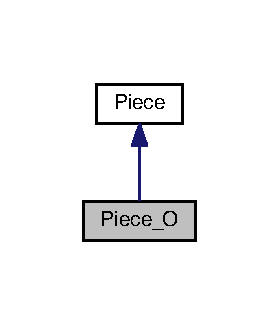
\includegraphics[width=134pt]{classPiece__O__inherit__graph}
\end{center}
\end{figure}


Collaboration diagram for Piece\+\_\+O\+:
\nopagebreak
\begin{figure}[H]
\begin{center}
\leavevmode
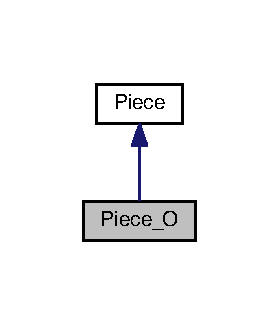
\includegraphics[width=134pt]{classPiece__O__coll__graph}
\end{center}
\end{figure}
\subsection*{Public Member Functions}
\begin{DoxyCompactItemize}
\item 
bool \hyperlink{classPiece__O_af82900ecec4e7bd058d43825293d8bff}{is\+Rotateable} (\hyperlink{classBoard}{Board} b)
\begin{DoxyCompactList}\small\item\em Vérifie si on peut tourner le Tétrimino en forme de carré d\textquotesingle{}un cran dans le sens horaire par rapport à la grille de jeu. \end{DoxyCompactList}\item 
void \hyperlink{classPiece__O_a69812f938582f176cd4cca997cbb87c1}{Rotate} (\hyperlink{classBoard}{Board} b)
\begin{DoxyCompactList}\small\item\em Permet la rotation d\textquotesingle{}un Tétrimino en forme de carré dans le sens horaire par rapport à la grille de jeu. Ne change rien en vu de la forme du Tétrimino. \end{DoxyCompactList}\item 
\mbox{\Hypertarget{classPiece__O_aa6abd4c92e4ca830993585f99b7d6a2a}\label{classPiece__O_aa6abd4c92e4ca830993585f99b7d6a2a}} 
\hyperlink{classPiece__O_aa6abd4c92e4ca830993585f99b7d6a2a}{Piece\+\_\+O} ()
\begin{DoxyCompactList}\small\item\em constructeur qui permet la création d\textquotesingle{}un Tétrimino en forme de carré, composé de 4 cases. A son initilisation, il est en position verticale. \end{DoxyCompactList}\end{DoxyCompactItemize}
\subsection*{Additional Inherited Members}


\subsection{Detailed Description}
Représentation d\textquotesingle{}un Tétrimino en forme de L. Hérite de Pièce. 

Représentation d\textquotesingle{}un Tétrimino en forme de carré. Hérite de Pièce.

\begin{DoxyAuthor}{Author}
Laura Couret 
\end{DoxyAuthor}
\begin{DoxyVersion}{Version}
1.\+0 
\end{DoxyVersion}
\begin{DoxyDate}{Date}
avril 2018 
\end{DoxyDate}
\begin{DoxyRefDesc}{Bug}
\item[\hyperlink{bug__bug000011}{Bug}]Rien à signaler \end{DoxyRefDesc}
\begin{DoxyWarning}{Warning}
Rien à signaler
\end{DoxyWarning}
Ce module permet la représentation physique d\textquotesingle{}un Tétrimino en forme de L. Cette classe hérite de Pièce, elle hérite donc de ses paramètres (couleur, etat, position, etc) et gardera ses méthodes de déplacement.

\begin{DoxyAuthor}{Author}
Léa Lefrançois 

Laura Couret 
\end{DoxyAuthor}
\begin{DoxyVersion}{Version}
1.\+0 
\end{DoxyVersion}
\begin{DoxyDate}{Date}
avril 2018 
\end{DoxyDate}
\begin{DoxyRefDesc}{Bug}
\item[\hyperlink{bug__bug000012}{Bug}]Rien à signaler \end{DoxyRefDesc}
\begin{DoxyWarning}{Warning}
Rien à signaler
\end{DoxyWarning}
Ce module permet la représentation physique d\textquotesingle{}un Tétrimino en forme de carré. Cette classe hérite de Pièce, elle hérite donc de ses paramètres (couleur, etat, position, etc) et gardera ses méthodes de déplacement. 

\subsection{Member Function Documentation}
\mbox{\Hypertarget{classPiece__O_af82900ecec4e7bd058d43825293d8bff}\label{classPiece__O_af82900ecec4e7bd058d43825293d8bff}} 
\index{Piece\+\_\+O@{Piece\+\_\+O}!is\+Rotateable@{is\+Rotateable}}
\index{is\+Rotateable@{is\+Rotateable}!Piece\+\_\+O@{Piece\+\_\+O}}
\subsubsection{\texorpdfstring{is\+Rotateable()}{isRotateable()}}
{\footnotesize\ttfamily bool Piece\+\_\+\+O\+::is\+Rotateable (\begin{DoxyParamCaption}\item[{\hyperlink{classBoard}{Board}}]{b }\end{DoxyParamCaption})\hspace{0.3cm}{\ttfamily [virtual]}}



Vérifie si on peut tourner le Tétrimino en forme de carré d\textquotesingle{}un cran dans le sens horaire par rapport à la grille de jeu. 


\begin{DoxyParams}{Parameters}
{\em b} & est la grille de notre Tetris \\
\hline
\end{DoxyParams}
\begin{DoxyReturn}{Returns}
renvoie vrai dans tous les cas car la rotation d\textquotesingle{}un carré ne change pas sa position dans la grille 
\end{DoxyReturn}


Implements \hyperlink{classPiece_a56cdf7f4234fe848a3e203b693b7a862}{Piece}.

\mbox{\Hypertarget{classPiece__O_a69812f938582f176cd4cca997cbb87c1}\label{classPiece__O_a69812f938582f176cd4cca997cbb87c1}} 
\index{Piece\+\_\+O@{Piece\+\_\+O}!Rotate@{Rotate}}
\index{Rotate@{Rotate}!Piece\+\_\+O@{Piece\+\_\+O}}
\subsubsection{\texorpdfstring{Rotate()}{Rotate()}}
{\footnotesize\ttfamily void Piece\+\_\+\+O\+::\+Rotate (\begin{DoxyParamCaption}\item[{\hyperlink{classBoard}{Board}}]{b }\end{DoxyParamCaption})\hspace{0.3cm}{\ttfamily [virtual]}}



Permet la rotation d\textquotesingle{}un Tétrimino en forme de carré dans le sens horaire par rapport à la grille de jeu. Ne change rien en vu de la forme du Tétrimino. 


\begin{DoxyParams}{Parameters}
{\em b} & est la grille de notre Tetris \\
\hline
\end{DoxyParams}


Implements \hyperlink{classPiece_a078f3cc6281cb8f60af3ae2266c651ba}{Piece}.



The documentation for this class was generated from the following files\+:\begin{DoxyCompactItemize}
\item 
Piece\+\_\+\+O.\+hpp\item 
Piece\+\_\+\+O.\+cpp\end{DoxyCompactItemize}

\hypertarget{classPiece__S}{}\section{Piece\+\_\+S Class Reference}
\label{classPiece__S}\index{Piece\+\_\+S@{Piece\+\_\+S}}


Représentation d\textquotesingle{}un Tétrimino en forme de S. Hérite de Pièce.  




{\ttfamily \#include $<$Piece\+\_\+\+S.\+hpp$>$}



Inheritance diagram for Piece\+\_\+S\+:
\nopagebreak
\begin{figure}[H]
\begin{center}
\leavevmode
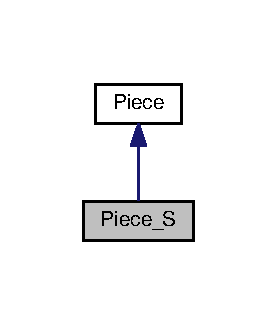
\includegraphics[width=133pt]{classPiece__S__inherit__graph}
\end{center}
\end{figure}


Collaboration diagram for Piece\+\_\+S\+:
\nopagebreak
\begin{figure}[H]
\begin{center}
\leavevmode
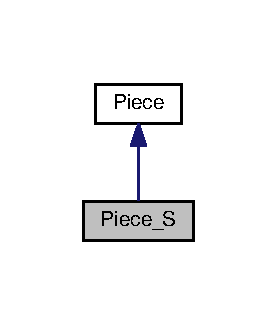
\includegraphics[width=133pt]{classPiece__S__coll__graph}
\end{center}
\end{figure}
\subsection*{Public Member Functions}
\begin{DoxyCompactItemize}
\item 
bool \hyperlink{classPiece__S_a725b9e7b154628e035bcc7ebd2a3ec9f}{is\+Rotateable} (\hyperlink{classBoard}{Board} b)
\begin{DoxyCompactList}\small\item\em Vérifie si on peut tourner le Tétrimino en forme de S d\textquotesingle{}un cran dans le sens horaire par rapport à la grille de jeu. \end{DoxyCompactList}\item 
void \hyperlink{classPiece__S_aefb2837f39f6b05bc678a3fdadc192b0}{Rotate} (\hyperlink{classBoard}{Board} b)
\begin{DoxyCompactList}\small\item\em Permet la rotation d\textquotesingle{}un Tétrimino en forme de S dans le sens horaire par rapport à la grille de jeu. \end{DoxyCompactList}\item 
\mbox{\Hypertarget{classPiece__S_aa39b8ee3dd219a03af2c6e0b3d05be5c}\label{classPiece__S_aa39b8ee3dd219a03af2c6e0b3d05be5c}} 
\hyperlink{classPiece__S_aa39b8ee3dd219a03af2c6e0b3d05be5c}{Piece\+\_\+S} ()
\begin{DoxyCompactList}\small\item\em constructeur qui permet la création d\textquotesingle{}un Tétrimino en forme de S, composé de 4 cases. A son initilisation, il est en position carrée mais avec la rangée supérieure décalée d\textquotesingle{}un cran vers la droite. \end{DoxyCompactList}\end{DoxyCompactItemize}
\subsection*{Additional Inherited Members}


\subsection{Detailed Description}
Représentation d\textquotesingle{}un Tétrimino en forme de S. Hérite de Pièce. 

\begin{DoxyAuthor}{Author}
Léa Lefrançois 
\end{DoxyAuthor}
\begin{DoxyVersion}{Version}
1.\+0 
\end{DoxyVersion}
\begin{DoxyDate}{Date}
avril 2018 
\end{DoxyDate}
\begin{DoxyRefDesc}{Bug}
\item[\hyperlink{bug__bug000013}{Bug}]Rien à signaler \end{DoxyRefDesc}
\begin{DoxyWarning}{Warning}
Rien à signaler
\end{DoxyWarning}
Ce module permet la représentation physique d\textquotesingle{}un Tétrimino en forme de S. Cette classe hérite de Pièce, elle hérite donc de ses paramètres (couleur, etat, position, etc) et gardera ses méthodes de déplacement. 

\subsection{Member Function Documentation}
\mbox{\Hypertarget{classPiece__S_a725b9e7b154628e035bcc7ebd2a3ec9f}\label{classPiece__S_a725b9e7b154628e035bcc7ebd2a3ec9f}} 
\index{Piece\+\_\+S@{Piece\+\_\+S}!is\+Rotateable@{is\+Rotateable}}
\index{is\+Rotateable@{is\+Rotateable}!Piece\+\_\+S@{Piece\+\_\+S}}
\subsubsection{\texorpdfstring{is\+Rotateable()}{isRotateable()}}
{\footnotesize\ttfamily bool Piece\+\_\+\+S\+::is\+Rotateable (\begin{DoxyParamCaption}\item[{\hyperlink{classBoard}{Board}}]{b }\end{DoxyParamCaption})\hspace{0.3cm}{\ttfamily [virtual]}}



Vérifie si on peut tourner le Tétrimino en forme de S d\textquotesingle{}un cran dans le sens horaire par rapport à la grille de jeu. 


\begin{DoxyParams}{Parameters}
{\em b} & est la grille de notre Tetris \\
\hline
\end{DoxyParams}


Implements \hyperlink{classPiece_a56cdf7f4234fe848a3e203b693b7a862}{Piece}.

\mbox{\Hypertarget{classPiece__S_aefb2837f39f6b05bc678a3fdadc192b0}\label{classPiece__S_aefb2837f39f6b05bc678a3fdadc192b0}} 
\index{Piece\+\_\+S@{Piece\+\_\+S}!Rotate@{Rotate}}
\index{Rotate@{Rotate}!Piece\+\_\+S@{Piece\+\_\+S}}
\subsubsection{\texorpdfstring{Rotate()}{Rotate()}}
{\footnotesize\ttfamily void Piece\+\_\+\+S\+::\+Rotate (\begin{DoxyParamCaption}\item[{\hyperlink{classBoard}{Board}}]{b }\end{DoxyParamCaption})\hspace{0.3cm}{\ttfamily [virtual]}}



Permet la rotation d\textquotesingle{}un Tétrimino en forme de S dans le sens horaire par rapport à la grille de jeu. 


\begin{DoxyParams}{Parameters}
{\em b} & est la grille de notre Tetris \\
\hline
\end{DoxyParams}


Implements \hyperlink{classPiece_a078f3cc6281cb8f60af3ae2266c651ba}{Piece}.



The documentation for this class was generated from the following file\+:\begin{DoxyCompactItemize}
\item 
Piece\+\_\+\+S.\+hpp\end{DoxyCompactItemize}

\hypertarget{classPiece__T}{}\section{Piece\+\_\+T Class Reference}
\label{classPiece__T}\index{Piece\+\_\+T@{Piece\+\_\+T}}


Représentation d\textquotesingle{}un Tétrimino en forme de T. Hérite de \hyperlink{classPiece}{Piece}.  




{\ttfamily \#include $<$Piece\+\_\+\+T.\+hpp$>$}



Inheritance diagram for Piece\+\_\+T\+:
\nopagebreak
\begin{figure}[H]
\begin{center}
\leavevmode
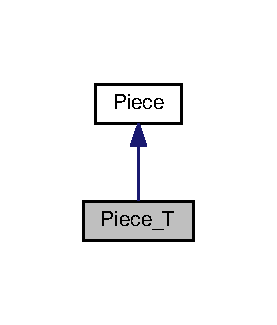
\includegraphics[width=133pt]{classPiece__T__inherit__graph}
\end{center}
\end{figure}


Collaboration diagram for Piece\+\_\+T\+:
\nopagebreak
\begin{figure}[H]
\begin{center}
\leavevmode
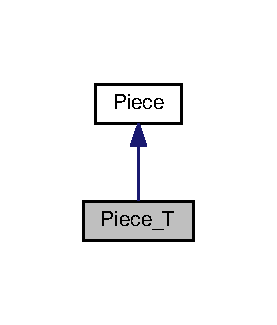
\includegraphics[width=133pt]{classPiece__T__coll__graph}
\end{center}
\end{figure}
\subsection*{Public Member Functions}
\begin{DoxyCompactItemize}
\item 
bool \hyperlink{classPiece__T_a64088f0140b870d178169e36460cd4de}{is\+Rotateable} (\hyperlink{classBoard}{Board} b)
\begin{DoxyCompactList}\small\item\em Vérifie si on peut tourner le Tétrimino en forme de T d\textquotesingle{}un cran dans le sens horaire par rapport au \hyperlink{classBoard}{Board}. \end{DoxyCompactList}\item 
void \hyperlink{classPiece__T_affedcbe550aebd2a9e8ec169d1fe0a9f}{Rotate} (\hyperlink{classBoard}{Board} b)
\begin{DoxyCompactList}\small\item\em Permet la rotation d\textquotesingle{}un Tétrimino en forme de T dans le sens horaire par rapport au \hyperlink{classBoard}{Board}. \end{DoxyCompactList}\item 
\mbox{\Hypertarget{classPiece__T_aa83bf987b663f99cc412f59ec08a94a1}\label{classPiece__T_aa83bf987b663f99cc412f59ec08a94a1}} 
\hyperlink{classPiece__T_aa83bf987b663f99cc412f59ec08a94a1}{Piece\+\_\+T} ()
\begin{DoxyCompactList}\small\item\em constructeur qui permet la création d\textquotesingle{}un Tétrimino en forme de T, composé de 4 cases \+: une ligne de 3 cases, et une case en dessous de la case du milieu de cette ligne. \end{DoxyCompactList}\end{DoxyCompactItemize}
\subsection*{Additional Inherited Members}


\subsection{Detailed Description}
Représentation d\textquotesingle{}un Tétrimino en forme de T. Hérite de \hyperlink{classPiece}{Piece}. 

\begin{DoxyAuthor}{Author}
Victor Le Maistre 
\end{DoxyAuthor}
\begin{DoxyVersion}{Version}
1.\+0 
\end{DoxyVersion}
\begin{DoxyDate}{Date}
avril 2018 
\end{DoxyDate}
\begin{DoxyRefDesc}{Bug}
\item[\hyperlink{bug__bug000016}{Bug}]Rien à signaler \end{DoxyRefDesc}
\begin{DoxyWarning}{Warning}
Rien à signaler
\end{DoxyWarning}
Ce module permet la représentation physique d\textquotesingle{}un Tétrimino en forme de T. Cette classe hérite de \hyperlink{classPiece}{Piece}, elle hérite donc de ses paramètres (couleur, etat, position, etc) et gardera ses méthodes de déplacement. 

\subsection{Member Function Documentation}
\mbox{\Hypertarget{classPiece__T_a64088f0140b870d178169e36460cd4de}\label{classPiece__T_a64088f0140b870d178169e36460cd4de}} 
\index{Piece\+\_\+T@{Piece\+\_\+T}!is\+Rotateable@{is\+Rotateable}}
\index{is\+Rotateable@{is\+Rotateable}!Piece\+\_\+T@{Piece\+\_\+T}}
\subsubsection{\texorpdfstring{is\+Rotateable()}{isRotateable()}}
{\footnotesize\ttfamily bool Piece\+\_\+\+T\+::is\+Rotateable (\begin{DoxyParamCaption}\item[{\hyperlink{classBoard}{Board}}]{b }\end{DoxyParamCaption})\hspace{0.3cm}{\ttfamily [virtual]}}



Vérifie si on peut tourner le Tétrimino en forme de T d\textquotesingle{}un cran dans le sens horaire par rapport au \hyperlink{classBoard}{Board}. 


\begin{DoxyParams}{Parameters}
{\em b} & est le \hyperlink{classBoard}{Board} de notre Tetris \\
\hline
\end{DoxyParams}
\begin{DoxyReturn}{Returns}
renvoie vrai si c\textquotesingle{}est possible, non sinon 
\end{DoxyReturn}


Implements \hyperlink{classPiece_a56cdf7f4234fe848a3e203b693b7a862}{Piece}.

\mbox{\Hypertarget{classPiece__T_affedcbe550aebd2a9e8ec169d1fe0a9f}\label{classPiece__T_affedcbe550aebd2a9e8ec169d1fe0a9f}} 
\index{Piece\+\_\+T@{Piece\+\_\+T}!Rotate@{Rotate}}
\index{Rotate@{Rotate}!Piece\+\_\+T@{Piece\+\_\+T}}
\subsubsection{\texorpdfstring{Rotate()}{Rotate()}}
{\footnotesize\ttfamily void Piece\+\_\+\+T\+::\+Rotate (\begin{DoxyParamCaption}\item[{\hyperlink{classBoard}{Board}}]{b }\end{DoxyParamCaption})\hspace{0.3cm}{\ttfamily [virtual]}}



Permet la rotation d\textquotesingle{}un Tétrimino en forme de T dans le sens horaire par rapport au \hyperlink{classBoard}{Board}. 


\begin{DoxyParams}{Parameters}
{\em b} & est le \hyperlink{classBoard}{Board} de notre Tetris \\
\hline
\end{DoxyParams}


Implements \hyperlink{classPiece_a078f3cc6281cb8f60af3ae2266c651ba}{Piece}.



The documentation for this class was generated from the following files\+:\begin{DoxyCompactItemize}
\item 
Piece\+\_\+\+T.\+hpp\item 
Piece\+\_\+\+T.\+cpp\end{DoxyCompactItemize}

\hypertarget{classPiece__Z}{}\section{Piece\+\_\+Z Class Reference}
\label{classPiece__Z}\index{Piece\+\_\+Z@{Piece\+\_\+Z}}


Représentation d\textquotesingle{}un Tétrimino en forme de J. Hérite de Pièce.  




{\ttfamily \#include $<$Piece\+\_\+\+Z.\+hpp$>$}



Inheritance diagram for Piece\+\_\+Z\+:
\nopagebreak
\begin{figure}[H]
\begin{center}
\leavevmode
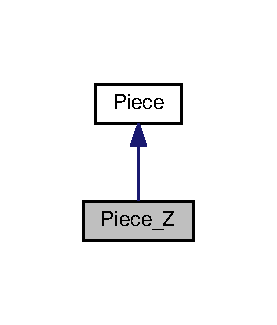
\includegraphics[width=133pt]{classPiece__Z__inherit__graph}
\end{center}
\end{figure}


Collaboration diagram for Piece\+\_\+Z\+:
\nopagebreak
\begin{figure}[H]
\begin{center}
\leavevmode
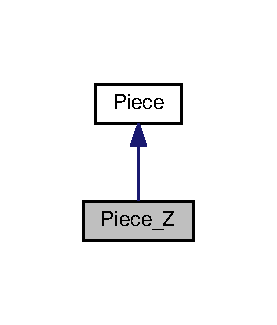
\includegraphics[width=133pt]{classPiece__Z__coll__graph}
\end{center}
\end{figure}
\subsection*{Public Member Functions}
\begin{DoxyCompactItemize}
\item 
bool \hyperlink{classPiece__Z_aa70256d6f49dacad685a15c5ae8df06d}{is\+Rotateable} (\hyperlink{classBoard}{Board} b)
\begin{DoxyCompactList}\small\item\em Vérifie si on peut tourner le Tétrimino en forme de Z d\textquotesingle{}un cran dans le sens horaire par rapport à la grille de jeu. \end{DoxyCompactList}\item 
void \hyperlink{classPiece__Z_a50d6c34030c7641b4827353b9b82a68e}{Rotate} (\hyperlink{classBoard}{Board} b)
\begin{DoxyCompactList}\small\item\em Permet la rotation d\textquotesingle{}un Tétrimino en forme de Z dans le sens horaire par rapport à la grille de jeu. \end{DoxyCompactList}\item 
\mbox{\Hypertarget{classPiece__Z_aecae5333fb48fae61d1b572b3282fc09}\label{classPiece__Z_aecae5333fb48fae61d1b572b3282fc09}} 
\hyperlink{classPiece__Z_aecae5333fb48fae61d1b572b3282fc09}{Piece\+\_\+Z} ()
\begin{DoxyCompactList}\small\item\em constructeur qui permet la création d\textquotesingle{}un Tétrimino en forme de Z, composé de 4 cases. A son initilisation, il est en position carrée mais avec la rangée supérieure décalée d\textquotesingle{}un cran vers la gauche. \end{DoxyCompactList}\end{DoxyCompactItemize}
\subsection*{Additional Inherited Members}


\subsection{Detailed Description}
Représentation d\textquotesingle{}un Tétrimino en forme de J. Hérite de Pièce. 

\begin{DoxyAuthor}{Author}
Léa Lefrançois 
\end{DoxyAuthor}
\begin{DoxyVersion}{Version}
1.\+0 
\end{DoxyVersion}
\begin{DoxyDate}{Date}
avril 2018 
\end{DoxyDate}
\begin{DoxyRefDesc}{Bug}
\item[\hyperlink{bug__bug000015}{Bug}]Rien à signaler \end{DoxyRefDesc}
\begin{DoxyWarning}{Warning}
Rien à signaler
\end{DoxyWarning}
Ce module permet la représentation physique d\textquotesingle{}un Tétrimino en forme de Z. Cette classe hérite de Pièce, elle hérite donc de ses paramètres (couleur, etat, position, etc) et gardera ses méthodes de déplacement. 

\subsection{Member Function Documentation}
\mbox{\Hypertarget{classPiece__Z_aa70256d6f49dacad685a15c5ae8df06d}\label{classPiece__Z_aa70256d6f49dacad685a15c5ae8df06d}} 
\index{Piece\+\_\+Z@{Piece\+\_\+Z}!is\+Rotateable@{is\+Rotateable}}
\index{is\+Rotateable@{is\+Rotateable}!Piece\+\_\+Z@{Piece\+\_\+Z}}
\subsubsection{\texorpdfstring{is\+Rotateable()}{isRotateable()}}
{\footnotesize\ttfamily bool Piece\+\_\+\+Z\+::is\+Rotateable (\begin{DoxyParamCaption}\item[{\hyperlink{classBoard}{Board}}]{b }\end{DoxyParamCaption})\hspace{0.3cm}{\ttfamily [virtual]}}



Vérifie si on peut tourner le Tétrimino en forme de Z d\textquotesingle{}un cran dans le sens horaire par rapport à la grille de jeu. 


\begin{DoxyParams}{Parameters}
{\em b} & est la grille de notre Tetris \\
\hline
\end{DoxyParams}


Implements \hyperlink{classPiece_a56cdf7f4234fe848a3e203b693b7a862}{Piece}.

\mbox{\Hypertarget{classPiece__Z_a50d6c34030c7641b4827353b9b82a68e}\label{classPiece__Z_a50d6c34030c7641b4827353b9b82a68e}} 
\index{Piece\+\_\+Z@{Piece\+\_\+Z}!Rotate@{Rotate}}
\index{Rotate@{Rotate}!Piece\+\_\+Z@{Piece\+\_\+Z}}
\subsubsection{\texorpdfstring{Rotate()}{Rotate()}}
{\footnotesize\ttfamily void Piece\+\_\+\+Z\+::\+Rotate (\begin{DoxyParamCaption}\item[{\hyperlink{classBoard}{Board}}]{b }\end{DoxyParamCaption})\hspace{0.3cm}{\ttfamily [virtual]}}



Permet la rotation d\textquotesingle{}un Tétrimino en forme de Z dans le sens horaire par rapport à la grille de jeu. 


\begin{DoxyParams}{Parameters}
{\em b} & est la grille de notre Tetris \\
\hline
\end{DoxyParams}


Implements \hyperlink{classPiece_a078f3cc6281cb8f60af3ae2266c651ba}{Piece}.



The documentation for this class was generated from the following file\+:\begin{DoxyCompactItemize}
\item 
Piece\+\_\+\+Z.\+hpp\end{DoxyCompactItemize}

\hypertarget{classScore}{}\section{Score Class Reference}
\label{classScore}\index{Score@{Score}}


Gestion des meilleurs scores des joueurs.  




{\ttfamily \#include $<$Score.\+hpp$>$}

\subsection*{Public Member Functions}
\begin{DoxyCompactItemize}
\item 
\hyperlink{classScore_a93772a8d3e8c9f71cd3e4a0bf74d9e78}{Score} (string ch)
\begin{DoxyCompactList}\small\item\em Constructeur d\textquotesingle{}un \hyperlink{classScore}{Score}. \end{DoxyCompactList}\item 
void \hyperlink{classScore_a6575097aed9e43ec2b8c5926e00134c1}{addscore} (int s)
\begin{DoxyCompactList}\small\item\em Ajoute un nouveau score au fichier des meilleurs scores. \end{DoxyCompactList}\item 
bool \hyperlink{classScore_aed385c5969860d59ca1477e2699c2f54}{meilleurescore} (int s)
\begin{DoxyCompactList}\small\item\em Vérifie si un joueur peut rentrer dans le palmares des 5 meilleurs scores. \end{DoxyCompactList}\end{DoxyCompactItemize}


\subsection{Detailed Description}
Gestion des meilleurs scores des joueurs. 

\begin{DoxyAuthor}{Author}
Laura Couret 
\end{DoxyAuthor}
\begin{DoxyVersion}{Version}
1.\+0 
\end{DoxyVersion}
\begin{DoxyDate}{Date}
avril 2018 
\end{DoxyDate}
\begin{DoxyRefDesc}{Bug}
\item[\hyperlink{bug__bug000016}{Bug}]Rien à signaler \end{DoxyRefDesc}
\begin{DoxyWarning}{Warning}
Rien à signaler
\end{DoxyWarning}
Ce module permet la gestion des meilleurs scores. Plus particulièrmeent, on pourra consulter les meilleurs scores déjà réalisés, et en ajouter un nouveau si nécessaire. 

\subsection{Constructor \& Destructor Documentation}
\mbox{\Hypertarget{classScore_a93772a8d3e8c9f71cd3e4a0bf74d9e78}\label{classScore_a93772a8d3e8c9f71cd3e4a0bf74d9e78}} 
\index{Score@{Score}!Score@{Score}}
\index{Score@{Score}!Score@{Score}}
\subsubsection{\texorpdfstring{Score()}{Score()}}
{\footnotesize\ttfamily Score\+::\+Score (\begin{DoxyParamCaption}\item[{string}]{ch }\end{DoxyParamCaption})}



Constructeur d\textquotesingle{}un \hyperlink{classScore}{Score}. 


\begin{DoxyParams}{Parameters}
{\em ch} & est le nom du fichier de score à créer (un pour la version classiquen, un pour la version montagnarde) \\
\hline
\end{DoxyParams}


\subsection{Member Function Documentation}
\mbox{\Hypertarget{classScore_a6575097aed9e43ec2b8c5926e00134c1}\label{classScore_a6575097aed9e43ec2b8c5926e00134c1}} 
\index{Score@{Score}!addscore@{addscore}}
\index{addscore@{addscore}!Score@{Score}}
\subsubsection{\texorpdfstring{addscore()}{addscore()}}
{\footnotesize\ttfamily Score\+::addscore (\begin{DoxyParamCaption}\item[{int}]{s }\end{DoxyParamCaption})}



Ajoute un nouveau score au fichier des meilleurs scores. 


\begin{DoxyParams}{Parameters}
{\em s} & est le score réalisé à ajouter \\
\hline
\end{DoxyParams}
\mbox{\Hypertarget{classScore_aed385c5969860d59ca1477e2699c2f54}\label{classScore_aed385c5969860d59ca1477e2699c2f54}} 
\index{Score@{Score}!meilleurescore@{meilleurescore}}
\index{meilleurescore@{meilleurescore}!Score@{Score}}
\subsubsection{\texorpdfstring{meilleurescore()}{meilleurescore()}}
{\footnotesize\ttfamily bool Score\+::meilleurescore (\begin{DoxyParamCaption}\item[{int}]{s }\end{DoxyParamCaption})}



Vérifie si un joueur peut rentrer dans le palmares des 5 meilleurs scores. 


\begin{DoxyParams}{Parameters}
{\em s} & est le score réalisé à comparer avec ceux déjà réalisé \\
\hline
\end{DoxyParams}
\begin{DoxyReturn}{Returns}
true s\textquotesingle{}il s\textquotesingle{}agit d\textquotesingle{}un nouveau meilleur score, false sinon 
\end{DoxyReturn}


The documentation for this class was generated from the following file\+:\begin{DoxyCompactItemize}
\item 
Score.\+hpp\end{DoxyCompactItemize}

%--- End generated contents ---

% Index
\backmatter
\newpage
\phantomsection
\clearemptydoublepage
\addcontentsline{toc}{chapter}{Index}
\printindex

\end{document}
